\chapter{Vapour-Liquid Equilibrium of Mixtures}\label{Chapter:VLE}


   \begin{LearningObjectivesBlock}{Learning Objectives}
      Upon completion of this chapter, you will be able to
        \begin{enumerate}
           \item Assess properties of real fluids through excess properties definitions; 
           \item Define phase and components molar fractions;
           \item Discuss chemical potential as a critical element for chemical equilibrium;
           \item Determine conditions for chemical equilibrium;
           \item Estimate phases, compositions and thermodynamic potentials in 2-/3-D phase diagrams;
           \item Identify and calculate bubble and dew points coordinates (\ie pressure, temperature and compositions);
           \item State Raoult's and Henry's laws;
           \item Formulate mass balance for VLE problems and estimate compositions at equilibrium.
        \end{enumerate}
\medskip
     Recommended reading: Chapters 10-11 of \citet{SmithVanNess_Book}, 8-10 of \cite{Sandler_Book}, 3-5 of \citet{Lue_Book}, 11 of \citet{Moran_Book} or 4-7 of \citet{Atkins_Book}.
   \end{LearningObjectivesBlock}


%%%%%%%%%%%%%%%%%%%%%%%%%%%%%%%%%%%%%%%%%%%%%%%%%%%%%%%%%%%%%%%%%
\begin{comment}
   \begin{LearningObjectivesBlock}{Learning Objectives}
      Upon completion of this chapter, you will be able to
        \begin{enumerate}
           \item {\bf Knowledge:} Define, Name, Select, State 
           \item {\bf Comprehension:} Describe, Identify, Discuss
           \item {\bf Application:} Apply, Demonstrate, Employ, Sketch
           \item {\bf Analysis:} Analyse, Compare, Calculate, Solve
           \item {\bf Synthesis:} Determine, Formulate
           \item {\bf Evaluation:} Assess, Check, Estimate, Compare, Measure, Monitor
        \end{enumerate}
\end{comment}
%%%%%%%%%%%%%%%%%%%%%%%%%%%%%%%%%%%%%%%%%%%%%%%%%%%%%%%%%%%%%%%%%

%%%% ETOC
\localtableofcontents
   

%%% SECTION
\section{Introduction}\label{Chapter:VLE:Section:Introduction}
Up to this point, we have only considered thermodynamic and volumetric properties of pure components at prescribed pressure and temperature conditions. However, most engineering applications deals with mixtures of components that may be present in single or multiple phases, \eg oil in reservoirs, naphtha distillation, steel processing etc. This chapter focuses on understanding PVT behaviour of mixtures and the conditions for vapour-liquid equilibrium (VLE).



%%% SECTION
\section{A Few Important Definitions}
In the previous chapters, we mostly focused on thermodynamic properties of systems containing pure chemical species. This chapter (and the remaining of this notes) will study systems with arbitrary number of components, and the quantification of each component at each phase (Gibbs phase rule, Section~\ref{Chapter:VolumetricPropertiesPureSubstances:Section:GibbsPhaseRule}, is fundamental to determine the number of degrees of freedom in two-phase system with arbitrary number of chemical species).\index{Phase rule}

%%% SUBSECTION
\subsection{Representing Compositions}\label{Chapter:VLE:Section:Compositions}
 For a mixture containing $\mathcal{C}$ chemical species, each of them with an arbitrary number of moles, $n_{i},\;\;\forall i\in\left\{1,2,\cdots,\mathcal{C}\right\}$,
\begin{subequations}
   \begin{enumerate}[a)]\index{Molar fraction}
       \item Molar (or mole) fraction $\left(x_{i}\right)$:
            \begin{eqnarray}
                x_{i} = \frc{n_{i}}{n},\label{Chapter:VLE:Eqn:MolarFraction}
            \end{eqnarray} 
            where $n=\summation[n_{i}]{i=1}{\mathcal{C}}$ is the total number of moles in the system. As the molar fraction is a normalised quantity, the following constraint is imposed:
            \begin{equation}
                  \summation[x_{i}]{i=1}{\mathcal{C}} = 1,\label{Chapter:VLE:Eqn:MolarFractionConstraint}
            \end{equation}
       \item (Average) Molar mass of mixtures:\index{Molar mass}\index{Molar weight|see {Molar mass}}
            \begin{equation}
                \overline{MW} = \summation[\left(x_{i} \cdot MW_{i}\right)]{i=1}{\mathcal{C}}\label{Chapter:VLE:Eqn:MolarMass}
            \end{equation}
         where $MW_{i}$ is the molecular mass (or molar weight) of species $i$.
   \end{enumerate}
\end{subequations}

%%% SUBSECTION
\subsection{Partial Molar Properties}\label{Chapter:VLE:Section:PartialMolarProperties}\index{Partial molar properties}
Many thermodynamic properties of {\it ideal solutions} do not change on mixing, for example, the volume of a mixture (assumed ideal) is equal to the sum of the volume of the original unmixed solutions. However, in real systems the volume and other properties, are not additive, \ie the volume of a mixture is not equal to the sum of the volumes of the individual pure components. {\it Partial molar properties} describe the behaviour of homogeneous multi-component systems. Thus, the concept of partial molar properties are crucial tool to assess individual contribution to thermodynamic properties of mixtures. In Section~\ref{Chapter:SolutionThermodynamics:Section:GibbsDuhem}, an expression will be developed to assess thermodynamic properties of solutions based on this concept. 

 Let's consider a homogeneous (\ie single phase) and open system with $\mathcal{C}$ chemical species that undertakes a change in composition. Thus, the total value of any extensive property $M^{\text{t}}\;\left(M\equiv V, U, H, S, G, A\right)$ is not only a function of pressure and temperature, but it also depends on the number of moles of each species in the system, therefore
  \begin{subequations}
     \begin{equation}
       M^{\text{t}} = nM = M\left(T,P,n_{1},n_{2},\cdots, n_{\mathcal{C}}\right).\label{Chapter:VLE:Eqn:PartialProperties1}
     \end{equation}
     The total derivative of this property, $M^{\text{t}}$, is,
     \begin{displaymath}  
        d(nM) = \Partial[(nM)]{P}{T,n}dP + \Partial[(nM)]{T}{P,n}dT + \Partial[(nM)]{n_{i}}{T,P,n_{j\ne i}}dn_{i},
     \end{displaymath}
     where the subscript $n$ in the partial derivatives indicates that the number of moles is kept constant, whereas $n_{j\ne i}$ indicates that the number of moles of all components, except component $i$, are kept constant. This expression can be simplified to be a function of the mole fraction, $x_{i}$,
     \begin{shaded}
        \begin{equation}  
           d(nM) = n\Partial[M]{P}{T,x}dP + n\Partial[M]{T}{P,x}dT + \summation[\overline{M}_{i}dn_{i}]{i}{},\label{Chapter:VLE:Eqn:PartialProperties2}
        \end{equation}
        where
        \begin{displaymath}
          \overline{M}_{i} = \Partial[(nM)]{n_{i}}{T,P,n_{j\ne i}},
        \end{displaymath}
        defines the {\it partial molar property} of species $i$ in solution, \ie the change of the total property $M^{\text{t}}$ of a mixture of $\mathcal{C}$ species resulting from the addition at constant $T$ and $P$ of infinitesimal amount of species $i$ to a prescribed amount of solution. We will discuss applications of partial molar properties in Chapter~\ref{Chapter:SolutionThermodynamics}.
     \end{shaded}
  \end{subequations}

%%% SUBSECTION
\subsection{Excess Properties}\label{Chapter:VLE:Section:ExcessProperties}\index{Excess properties|see {Solutions}}\index{Solutions!Excess properties}
  
In Section~\ref{Chapter:ThermodynamicPropertiesPureFluids:Section:ResidualProperties}, {\it residual properties} were defined as the difference between any extensive thermodynamic property, $M$, in real gases and its equivalent assuming ideal gas behaviour, $M^{\text{ig}}$. This entity is only applied to gases, an equivalent for liquids is called {\it excess properties}, \ie the deviation from an ideal liquid solution property\footnote{A formal definition of ideal solutions will be seen in Section~\ref{Chapter:SolutionThermodynamics:Section:IdealSolution}.}.\index{Gases!Residual properties}\

Let's assume that $M$ is any extensive thermodynamic property (\eg $V$, $U$, $H$, $S$, $G$ and $A$), the excess property $M^{\text{E}}$ is defined as the difference between the property value of a solution and the value it would have as an ideal solution at the same $T$, $P$ and composition,
\begin{subequations}
  \begin{shaded}
    \begin{equation}
       M^{\text{E}} \equiv M - M^{\text{id}},\label{Chapter:VLE:Eqn:ExcessProperties1a}
    \end{equation}
  \end{shaded}
  \noindent where properties in ideal ({\it id}) solutions of multiple chemical species can be represented as,
    \begin{displaymath}
       M^{\text{id}} = \summation[x_{i}M_{i}]{i}{},
    \end{displaymath}
    where $M_{i}$ is an extensive molar property of the \underline{pure} chemical species. For example, if we mix equal volumes of two species (\eg water and ethanol), the final volume \underline{is not} the sum of the individual volumes. In fact, the final volume will be slightly larger than the sum of the individual volumes and this is due to the non-ideality behaviour of real liquid fluids. Thus for a binary solution ($\mathcal{C}=$ 2),
    \begin{shaded}
      \begin{equation}
        V^{\text{E}} = V - V^{\text{id}} = V - \summation[x_{i}V_{i}]{i}{} = V -\left(x_{1}V_{1}+x_{2}V_{2}\right).\label{Chapter:VLE:Eqn:ExcessProperties1b} 
      \end{equation}
      This equation shows that the total volume of a mixture of two components is different from the simple addition of both individual volumes.
    \end{shaded}
\end{subequations}
  
%%% SECTION
\section{Chemical Potential $\left(\mu_{i}\right)$}\label{Chapter:VLE:Section:ChemicalPotential}\index{Chemical potential}
  \begin{subequations}
If we apply the concept of partial molar property to the Gibbs free energy definition, assuming that this thermodynamic potential is a function of $P$, $T$ and $n$, \ie $G^{\text{t}}= nG = G\left(T,P,n_{1},n_{2},\cdots,n_{\mathcal{C}}\right)$,
      \begin{equation}
         d(nG) = n\Partial[G]{P}{T,x}dP + n\Partial[G]{T}{P,x}dT + \summation[\overline{G}_{i}dn_{i}]{i}{}.\label{Chapter:VLE:Eqn:ChemPotentialDef1}
      \end{equation}
      By definition the {\it partial molar Gibbs free energy} is called chemical potential $\left(\mu_{i}\right)$,
      \begin{shaded}
         \begin{equation}
            \overline{G}_{i} = \mu_{i} = \Partial[(nG)]{n_{i}}{T,P,n_{j\ne i}}. \label{Chapter:VLE:Eqn:ChemPotentialDef1b}
         \end{equation}
      \end{shaded}
      The chemical potential can be understood as an energy associated with interactions of atoms/molecules in a mixture that controls the tendency of molecules to either leave the liquid solution (towards the vapour phase) or return to the solution (from the vapour phase) to vapour phase, and to chemically react. The Gibbs free energy was defined in Eqn.~\ref{Chapter:ThermodynamicPropertiesPureFluids:Eqn:GibbsFundamentalRelation01} as a function of $T$ and $P$, now it can be extended to be also a function of the number of moles of the existing chemical species, and Eqn.~\ref{Chapter:VLE:Eqn:ChemPotentialDef1} becomes,
      \begin{equation}
         d(nG) = (nV)dP - (nS)dT + \summation[\mu_{i}dn_{i}]{i}{},\label{Chapter:VLE:Eqn:ChemPotentialDef1c}
      \end{equation}
      using Eqns.~\ref{Chapter:ThermodynamicPropertiesPureFluids:Eqn:MaxwellRelation7}-\ref{Chapter:ThermodynamicPropertiesPureFluids:Eqn:MaxwellRelation8}. Now, assuming $n=1\;\Rightarrow n_{i}=x_{i}$, and Eqn.~\ref{Chapter:VLE:Eqn:ChemPotentialDef1c} becomes
      \begin{shaded}
        \begin{equation}
          dG = VdP -SdT + \summation[\mu_{i}dx_{i}]{i}{},\label{Chapter:VLE:Eqn:ChemPotentialDef1d}
        \end{equation}
      \end{shaded}
  \end{subequations}
  
%%% SECTION
  \section{Criteria for Chemical Equilibrium}\label{Chapter:VLE:Section:ChemicalEquilibrium}
  
  %%% SUBSECTION
  \subsection{Thermodynamic Equilibrium}\label{Chapter:VLE:Section:ThermodynamicEquilibrium}
  \begin{subequations}
    There are two main conditions for a system to achieve chemical equilibrium:
    \begin{enumerate}[a)]
      \item all distinct $\mathcal{P}$ phases that may co-exist are in equilibrium with each other, as such as there is no net mass transfer of any chemical species between phases;
      \item all chemical reactions that may occur between species are also in equilibrium, \ie there is no net progress \wrt conversion of reactants to products (and vice-versa).
    \end{enumerate}

    Let's initially consider a closed system, either homogeneous or heterogeneous (\ie $\mathcal{P}\ge 1$), in thermal and mechanical equilibrium with the surroundings. In addition, let's also assume that the system is not under chemical equilibrium, \ie there are effective mass transfer across the phase boundaries. Such transfer of matter continues until the system reaches chemical equilibrium. In reality, these changes towards chemical equilibrium occur by infinitesimal gradients and are, therefore, irreversible. Applying the {\it First Law},
    \begin{displaymath}
      dU^{\text{t}} = dQ + dW\;\;\;\text{ with }\;\;\; dW = -PdV^{\text{t}},
    \end{displaymath}
    with the heat exchange between the system and the surroundings,
    \begin{displaymath}
      dS_{\text{surr}} = \frc{dQ_{\text{surr}}}{T_{\text{surr}}} = - \frc{dQ^{\text{t}}}{T},\;\;\text{ where } dQ_{\text{surr}} = - dQ^{\text{t}}.
    \end{displaymath}
    However, by the Second Law, $dS_{\text{surr}}+dS^{\text{t}} \ge 0$ (Eqn.~\ref{Chapter:SecondLaw:Eqn:Entropy2}), and if we combine the expressions above,
    \begin{displaymath}
       - \frc{dQ^{\text{t}}}{T}+dS^{\text{t}}\ge 0 \;\;\;\Longrightarrow\;\;\;  dQ^{\text{t}} \leq TdS^{\text{t}},
    \end{displaymath}
    \ie for every allowed change in state, the system can not spontaneously leave the current state. Thus, the system is said to be at \underline{stable equilibrium}.
    \begin{shaded}
      The \underline{entropy} of an adiabatically (\ie $dS<0$) isolated stable equilibrium system is \underline{maximum}.
    \end{shaded}
    We can write the criterion for stable equilibrium in non-adiabatic system from the First Law for $n$ moles,
    \begin{eqnarray}
      dQ = dU + PdV -\mu dn &\leq& TdS \label{Chapter:VLE:Eqn:EquilibriumCriteria0} \\
      dU + PdV -\mu dn - TdS &\leq& 0,\label{Chapter:VLE:Eqn:EquilibriumCriteria1}
    \end{eqnarray}
    thus,
    \begin{enumerate}[i)]
        \item if $U$, $V$ and $n$ are assumed constants: $dQ=0$ and the stability condition becomes $dS \ge 0$ $\Longrightarrow$ \underline{$S$ is maximum};
        \item if $S$, $V$ and $n$ are assumed constants: from Eqn.~\ref{Chapter:VLE:Eqn:EquilibriumCriteria1}, the system will be stable if $dU\le 0$ $\Longrightarrow$ \underline{$U$ is minimum};
        \item if $T$, $V$ and $n$ are assumed constants: Eqn.~\ref{Chapter:VLE:Eqn:EquilibriumCriteria1}, becomes
            \begin{eqnarray}
              dU - TdS &\leq& 0 \nonumber \\
              d(U-TS) &\leq& 0 \;\;  \text{(for } T \text{  constant}),
            \end{eqnarray}
            however, from the definition of the Helmholtz free energy, $U-TS =A$ (Section~\ref{Chapter:ThermodynamicPropertiesPureFluids:Section:ThermodynamicPropertiesSinglePhase}), thus $dA\leq0$ $\Longrightarrow$ \underline{$A$ is minimum};
        \item from the Helmholtz free energy definition,
            \begin{eqnarray}
               dA &=& \overbrace{dU}^{\text{from Eqn.~\ref{Chapter:VLE:Eqn:EquilibriumCriteria0}}: dU = dQ -dW +\mu dn} -SdT - TdS \nonumber \\
                  &=& dQ -dW + \mu dn -SdT -TdS,\label{Chapter:VLE:Eqn:EquilibriumCriteria2}
            \end{eqnarray}
            from the Clausius inequality (Section~\ref{Chapter:SecondLaw:Section:SecondLawStatement_Maths}), $dQ-TdS \leq 0$, and if $T$ and $n$ are assumed constants $\Longrightarrow\;\; dA = -dW + (dQ - TdS) \leq 0$, therefore
            \begin{displaymath}
                 dA \leq -dW \;\;\;\text{ or }\;\;\; W \leq -\Delta A.
            \end{displaymath}
            This means that $-\Delta A$ is the maximum work that can be obtained from a process performed under constant $T$ and $n$ conditions. Also, as $A$ is a \underline{state function}, it does \underline{not} depend on the path, but only on the initial and final states;
         \item if $S$, $P$ and $n$ are assumed constants: Eqn.~\ref{Chapter:VLE:Eqn:EquilibriumCriteria1} becomes
            \begin{displaymath}
                 d(U+PV) = dH \leq 0,
            \end{displaymath}
            for stable equilibrium $\Longrightarrow$ \underline{enthalpy is minimum};
         \item if $T$, $P$ and $n$ are assumed constants: Eqn.~\ref{Chapter:VLE:Eqn:EquilibriumCriteria1} becomes,
            \begin{displaymath}
                 d(U+PV-TS)  \leq 0,
            \end{displaymath}
            but $U+PV-TS = H-TS = G$, \ie \underline{the Gibbs free energy is minimum} for stable equilibrium with fixed $T$, $P$ and $n$.    
    \end{enumerate}
    In Table~\ref{Chapter:VLE:Table:TableEquilibriumCriteria}, the equilibrium criteria is summarised for all thermodynamic potentials. The stability criteria for the Gibbs free energy is particularly important for several chemical engineering processes involving closed systems, as so as we can state,
    \begin{shaded}
         `The equilibrium state of a closed system is that state for which the total Gibbs free energy is a minimum \wrt all possible changes at the given $T$ and $P$.'
      \end{shaded}

%%% TABLE   
    \begin{table}
    \begin{center}
      \begin{tabular}{c c c c c}
         \hline
          Held            & State    &  Definition & Differential         &  Stable Equilibrium \\
          Fixed           & Function &             &                      &   Criterion          \\
          \hline
          $U$, $V$, $n$   & $S$      & --          & $dS=\frac{dQ}{T}$    & Maximum             \\
          $S$, $V$, $n$   & $U$      & --          & $dU=TdS-PdV+\mu dn$ & Minimum             \\
          $S$, $P$, $n$   & $H$      & $H\equiv U+PV$& $dH=TdS+VdP+\mu dn$ & Minimum             \\
          $T$, $V$, $n$   & $A$      & $A\equiv U-TS$& $dA=-SdT-PdV+\mu dn$ & Minimum             \\
          $T$, $P$, $n$   & $G$      & $G\equiv H-TS$& $dG=-SdT+VdP+\mu dn$ & Minimum             \\
          \hline
      \end{tabular}
    \end{center}
    \caption{Criteria for thermodynamic equilibria.}\label{Chapter:VLE:Table:TableEquilibriumCriteria}
    \end{table}
    
  \end{subequations}

%%% SUBSECTION
\subsection{Chemical Potential and Thermodynamic Equilibrium}\label{Chapter:VLE:Section:ChemPotThermEquil}
  \begin{subequations}
    Now, let's consider a closed system consisting of two phases in equilibrium (\ie $\mathcal{P}=$ 2, \eg vapour and liquid, or solid and vapour or liquid and solid), $\alpha$ and $\beta$. Each of these phases may be considered as an open system with an interface between them, where mass and energy can flow freely. Also, both systems (or phases) are in mechanical and thermal equilibrium, \ie
    \begin{displaymath}
      \begin{cases}
        T^{\alpha}=T^{\beta}=T & \text{ and } \\
        P^{\alpha}=P^{\beta}=P,
      \end{cases}
    \end{displaymath}
    and Eqn~\ref{Chapter:VLE:Eqn:ChemPotentialDef1c} can be applied to both phases,
    \begin{eqnarray}
        d(nG)^{\alpha} &=& (nV)^{\alpha}dP - (nS)^{\alpha}dT + \summation[\mu_{i}^{\alpha}dn_{i}^{\alpha}]{i}{},\label{Chapter:VLE:Eqn:ChemPotentialDef1c1} \\
        d(nG)^{\beta} &=& (nV)^{\beta}dP - (nS)^{\beta}dT + \summation[\mu_{i}^{\beta}dn_{i}^{\beta}]{i}{}.\label{Chapter:VLE:Eqn:ChemPotentialDef1c2} 
    \end{eqnarray}
     The change in total Gibbs free energy of a two-phase system is the sum of the changes in each phase. As mass is transferred across the interface, volume and entropy of each phase may change,
     \begin{displaymath}
       \begin{cases}
         (nV) = (nV)^{\alpha}+ (nV)^{\beta} &  \\
         (nS) = (nS)^{\alpha}+(nS)^{\beta},&
       \end{cases}
     \end{displaymath}
     Summing up Eqns.~\ref{Chapter:VLE:Eqn:ChemPotentialDef1c1} and~\ref{Chapter:VLE:Eqn:ChemPotentialDef1c2} and using the above relations,
     \begin{displaymath}
        d(nG) = (nV)dP - (nS)dT + \summation[\mu_{i}^{\alpha}dn_{i}^{\alpha}]{i}{} + \summation[\mu_{i}^{\beta}dn_{i}^{\beta}]{i}{} = 0,
     \end{displaymath}
     and as the whole system is closed and the net mass transfer is zero, \ie $dn_{i}^{\alpha}=-dn_{i}^{\beta}$ thus,
     \begin{displaymath}
        d(nG) = (nV)dP - (nS)dT + \summation[\left(\mu_{i}^{\alpha}-\mu_{i}^{\beta}\right)dn_{i}^{\alpha}]{i}{} = 0.
     \end{displaymath}
     \begin{shaded}
       \noindent As the system is assumed to be already under mechanical and thermal equilibrium (\ie $P$ and $T$ are constants),
       \begin{equation}
         \summation[\left(\mu_{i}^{\alpha}-\mu_{i}^{\beta}\right)dn_{i}^{\alpha}]{i}{} = 0,
       \end{equation}
       This equation describes changes in the chemical potential and in the mass of each component in each phase. In fact, throughout this derivation, $dn_{i}^{\alpha}$ is enforced to be independent of each other and therefore \underline{can not be zero}, hence
       \begin{equation}
         \mu_{i}^{\alpha} = \mu_{i}^{\beta}, \;\;\;\;\forall i=1,2,\cdots, \mathcal{C}.\label{Chapter:VLE:Eqn:ChemPotentialDef1c3} 
       \end{equation}
       This rather simple relation is crucial for understanding phase equilibria, as it states that for an arbitrary closed system at fixed $T$, $P$, thermodynamic equilibrium will be reached when the chemical potential of \underline{all} chemical species in one of the phases is \underline{equal} to the counterpart in the other phase. In fact, this argument can be extended for any number of phases (\ie $\mathcal{P}\ge 2$), \ie
       \begin{equation}
          \blue{\mu_{i}^{\alpha} = \mu_{i}^{\beta} = \cdots = \mu_{i}^{\mathcal{P}}, \hspace{2cm} \forall i=1,2,\cdots, \mathcal{C}.}\label{Chapter:VLE:EqnChemPotentialDef1c3} 
       \end{equation}
      \end{shaded}

  \end{subequations}

%%% SECTION
\section{Vapour-Liquid Equilibrium}\label{Chapter:VLE:Section:VLE}
One of the main objectives of Chapter~\ref{Chapter:VolumetricPropertiesPureSubstances} was to study the thermodynamic equilibrium of pure components that involved phase change (see Figs.~\ref{Chapter:VolumetricPropertiesPureSubstances:Fig:PVT_Surfaces}-\ref{Chapter:VolumetricPropertiesPureSubstances:Fig:PV-PT_Diagrams}), and in particular for vapour-liquid equilibrium (VLE). $PVT$ relations of pure components were quantitatively expressed through equations of state. In this section, the investigation of VLE will be extended to mixtures of arbitrary number of components. \ie $\mathcal{P}=$2 and $\mathcal{C}\ge$ 2.
%%%% FIGURE
      \begin{figure}[h]
         \begin{center}
           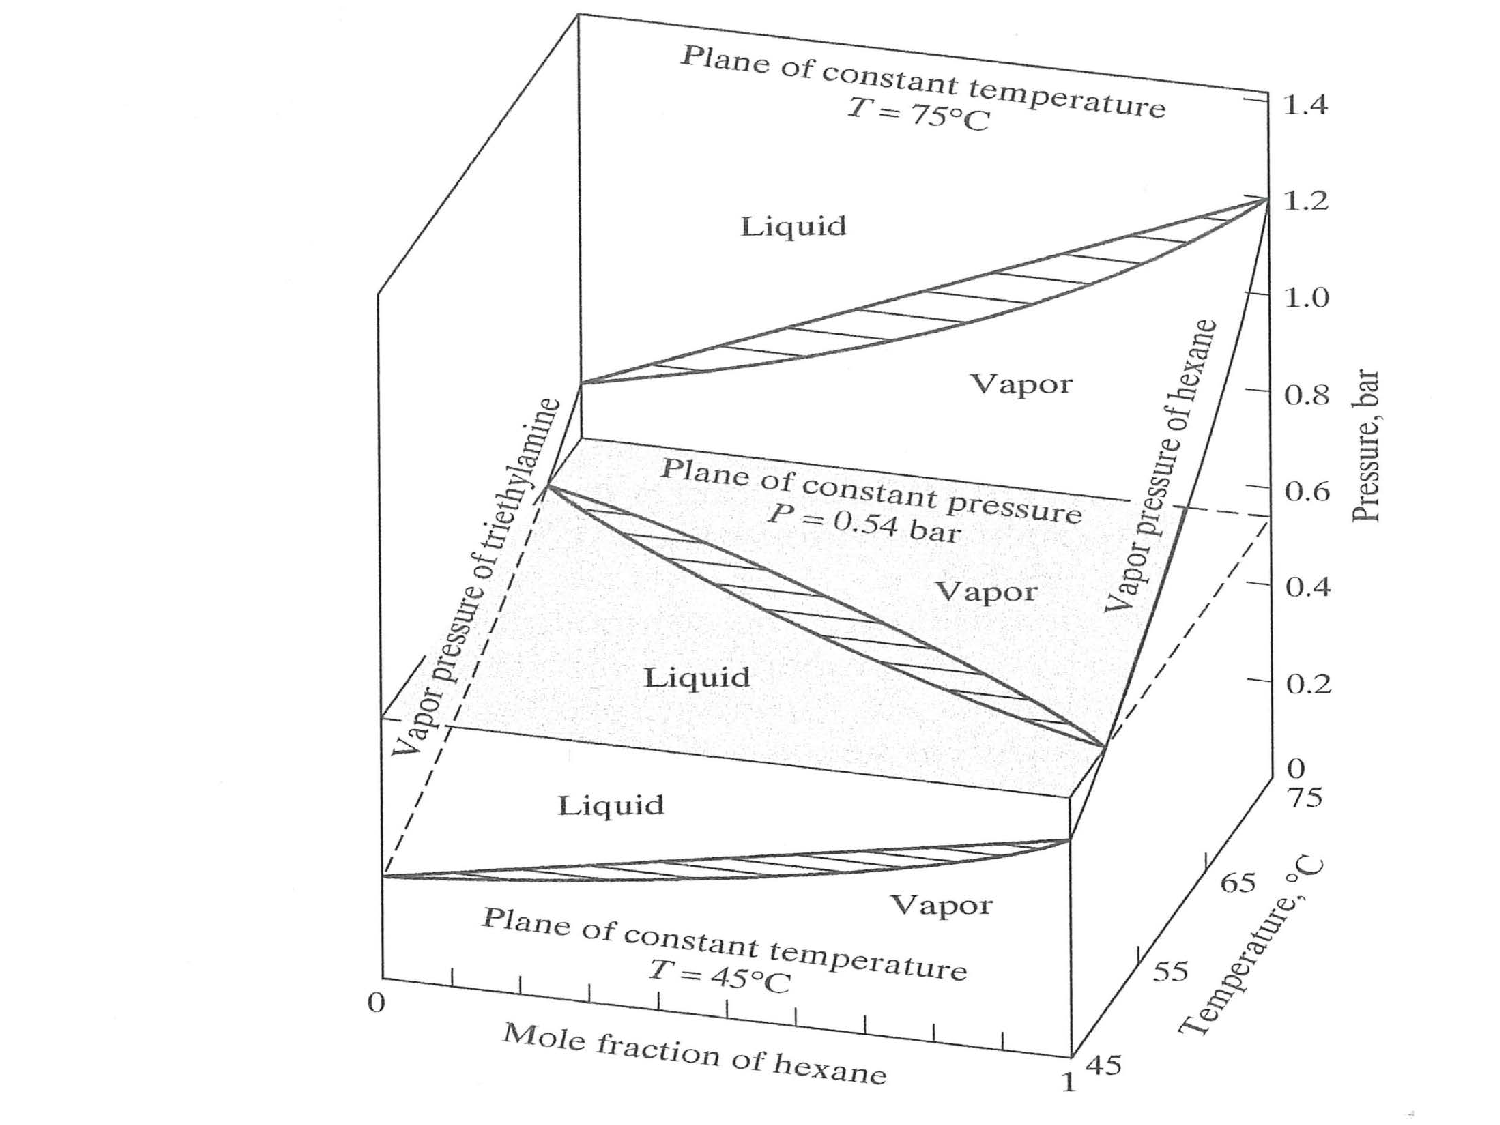
\includegraphics[width=.9\columnwidth,clip]{./../Pics/PTxy_diagram}
           \vspace{-.1cm}\caption{$P-T-xy$ diagram for hexane and triethylamine \citep[extracted from][]{Sandler_Book}.}\label{Chapter:VLE:Fig:Fig01}
         \end{center}
       \end{figure}

%%% SUBSECTION
\subsection{Qualitative Analysis: Phase Diagrams}\label{Chapter:VLE:Section:PhaseDiagrams}
In Section~\ref{Chapter:VolumetricPropertiesPureSubstances:Section:PVTBehaviour}, the {\it Gibbs phase rule} was introduced to help determining the number of degrees of freedom of any system,\index{Phase rule}\index{Phase rule !Degrees of freedom}
    \begin{displaymath}
        \Psi = 2 + \mathcal{C} - \mathcal{P}.
    \end{displaymath}
For a binary system in equilibrium (\ie $\mathcal{C}=2$), the phase rule yields a degree of freedom of $\Psi=4-\mathcal{P}$. In VLE systems ($\mathcal{P}=2$), the number of independent intensive variables becomes 2, and it will need to be chosen between:
\begin{enumerate}[a)]
   \item temperature ($T$);
   \item pressure ($P$);
   \item molar fraction of the more volatile component\footnote{In this chapter, for a mixture of $\mathcal{C}$ chemical species, the most volatile component will be assigned as number 1. Also, we will follow here the notation used in most thermodynamic text-books in which the molar fraction of component $i$ in vapour and liquid phases are \blue{$y_{i}$} and \blue{$x_{i}$}, respectively.} in the vapour phase $\left(y_{1}\right)$, and;
   \item molar fraction of the more volatile component in the liquid phase $\left(x_{1}\right)$.
\end{enumerate}
As shown in Fig.~\ref{Chapter:VLE:Fig:Fig01}, a plot with these 4 variables for a mixture of hexane and triethylamine is not very practical. In this $P-T-xy$ diagram, to ensure a single phase system $\left(\mathcal{P}=1\right)$, temperature, pressure and {\bf one} molar fraction need to be fixed. For a two-phase system $\left(\mathcal{P}=2\right)$, two variables need to be fixed and the system is expressed as a surface -- \eg the plane of constant pressure of $0.54$ bar. %Although insightful, this plot is not very convenient to assess compositions and phase behaviour, and is limited to a binary systems.
%%%% FIGURE
      \begin{figure}[h] 
         \begin{center}
             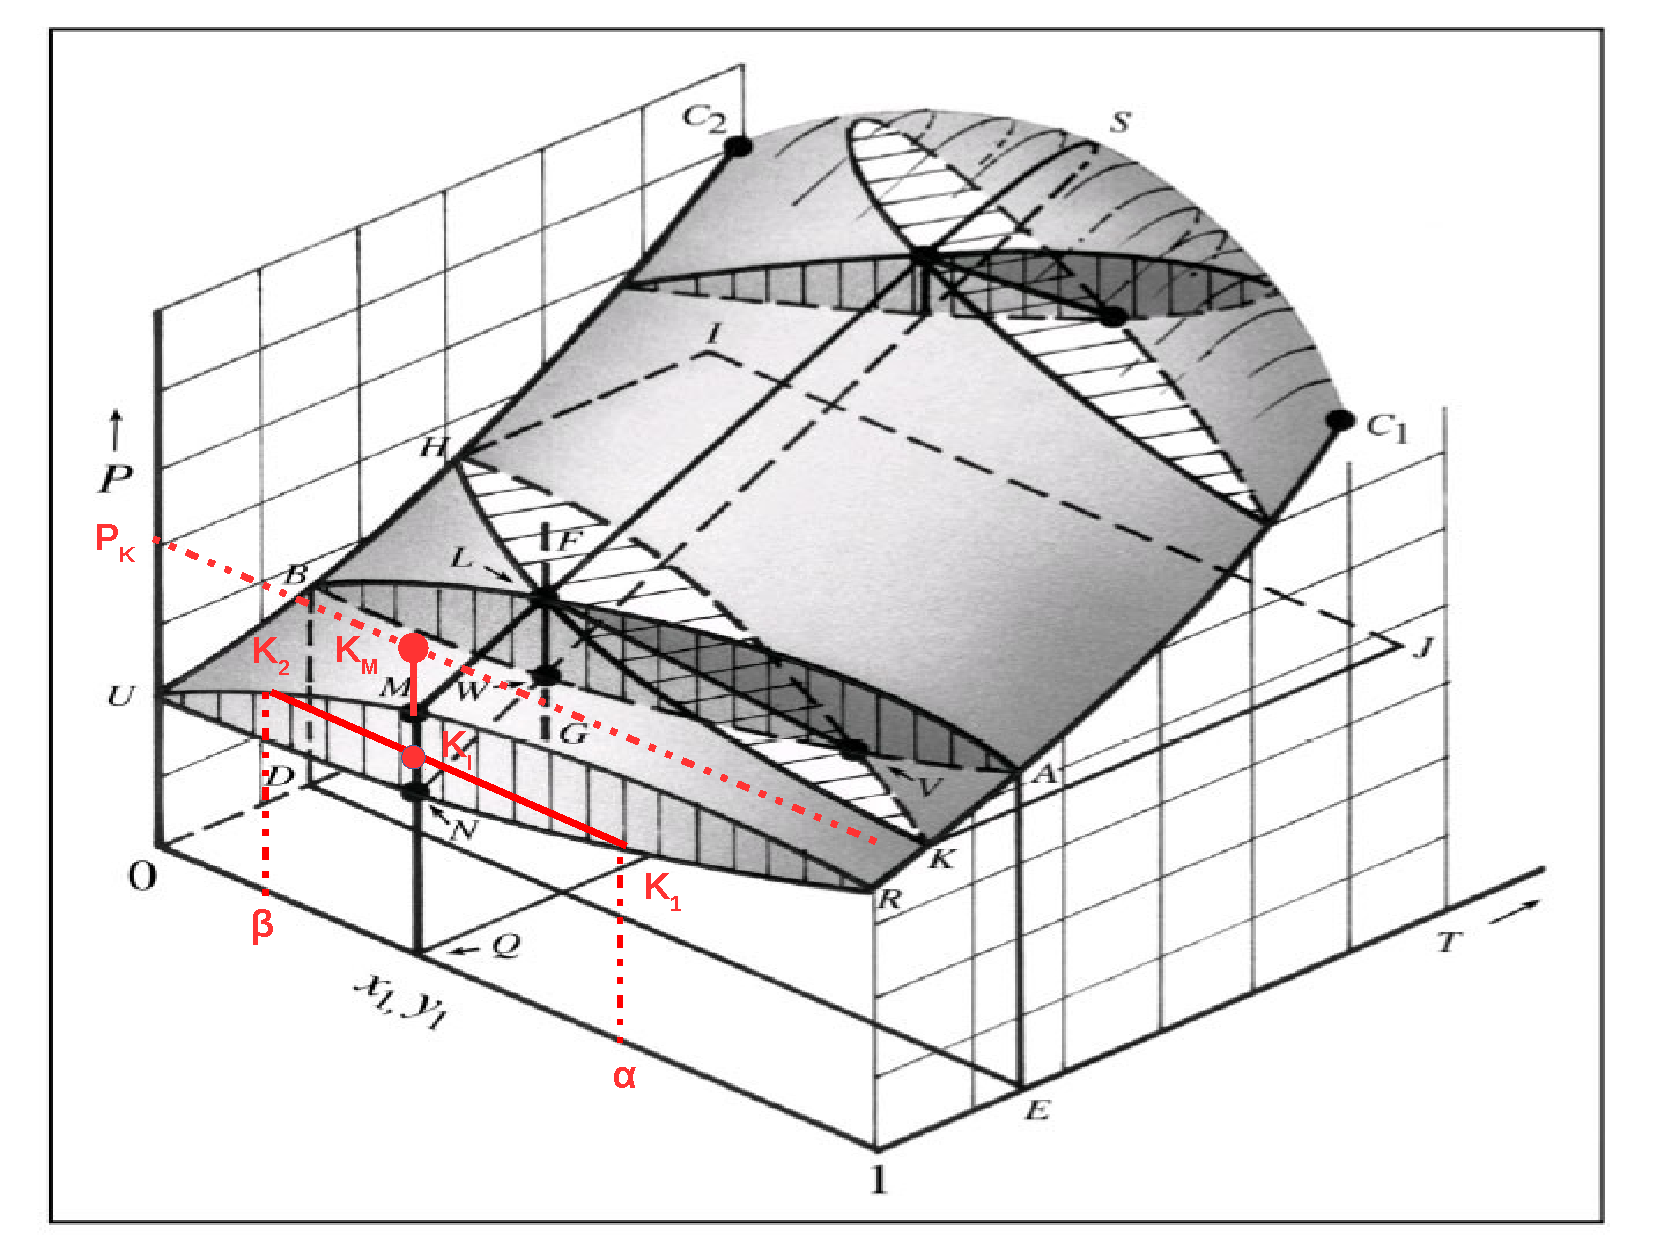
\includegraphics[width=.75\columnwidth,clip]{./Figs/PTxy_Digram} 
             \vspace{-.1cm}\caption{$P-T-xy$ diagram for binary mixtures \citep[extracted from][]{SmithVanNess_Book}.}\label{Chapter:VLE:Fig:Fig02}
         \end{center}
       \end{figure}

In a generic $P-T-xy$ diagram (Fig.~\ref{Chapter:VLE:Fig:Fig02}), vertical planes parallel to the \blue{0-1-R-M-U-0} plane (\eg plane \blue{E-A-B-D-E}) indicates $P-xy$ diagrams at constant temperature, whereas horizontal planes parallel to the \blue{K-J-I-H-K} plane indicates $T-xy$ diagrams at constant pressure. The liquid (\ie subcooled) region lies \underline{above} the upper-surface of the solid (grey) projection (solid body bounded by \blue{U-R-C$_{1}$-C$_{2}$-U}), and (superheated) vapour region lies \underline{below} the under-surface. The interior of the solid projection between the two surfaces is the region of coexistence of both liquid and vapour phases. 
%%% FIGURE
      \begin{figure}[h]
        \vbox{\hbox{\hspace{0.cm}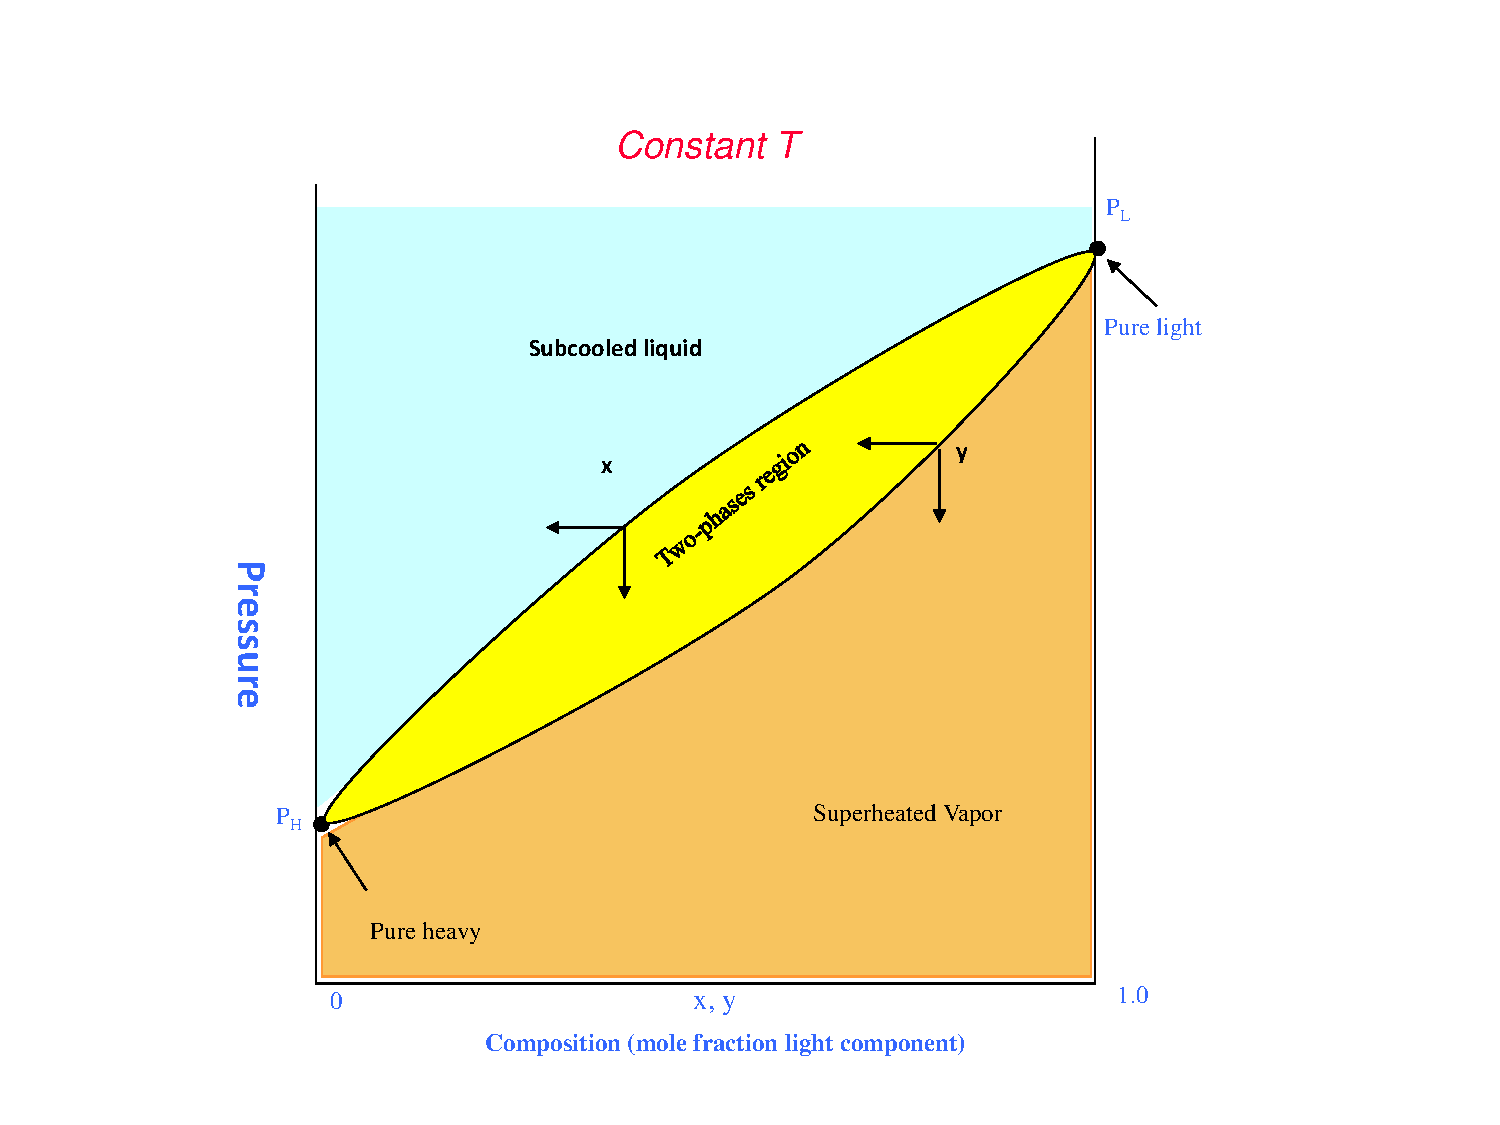
\includegraphics[width=.5\linewidth,clip]{./../Pics/VLE_Pxy_Diagram1}
            \hspace{-2.cm}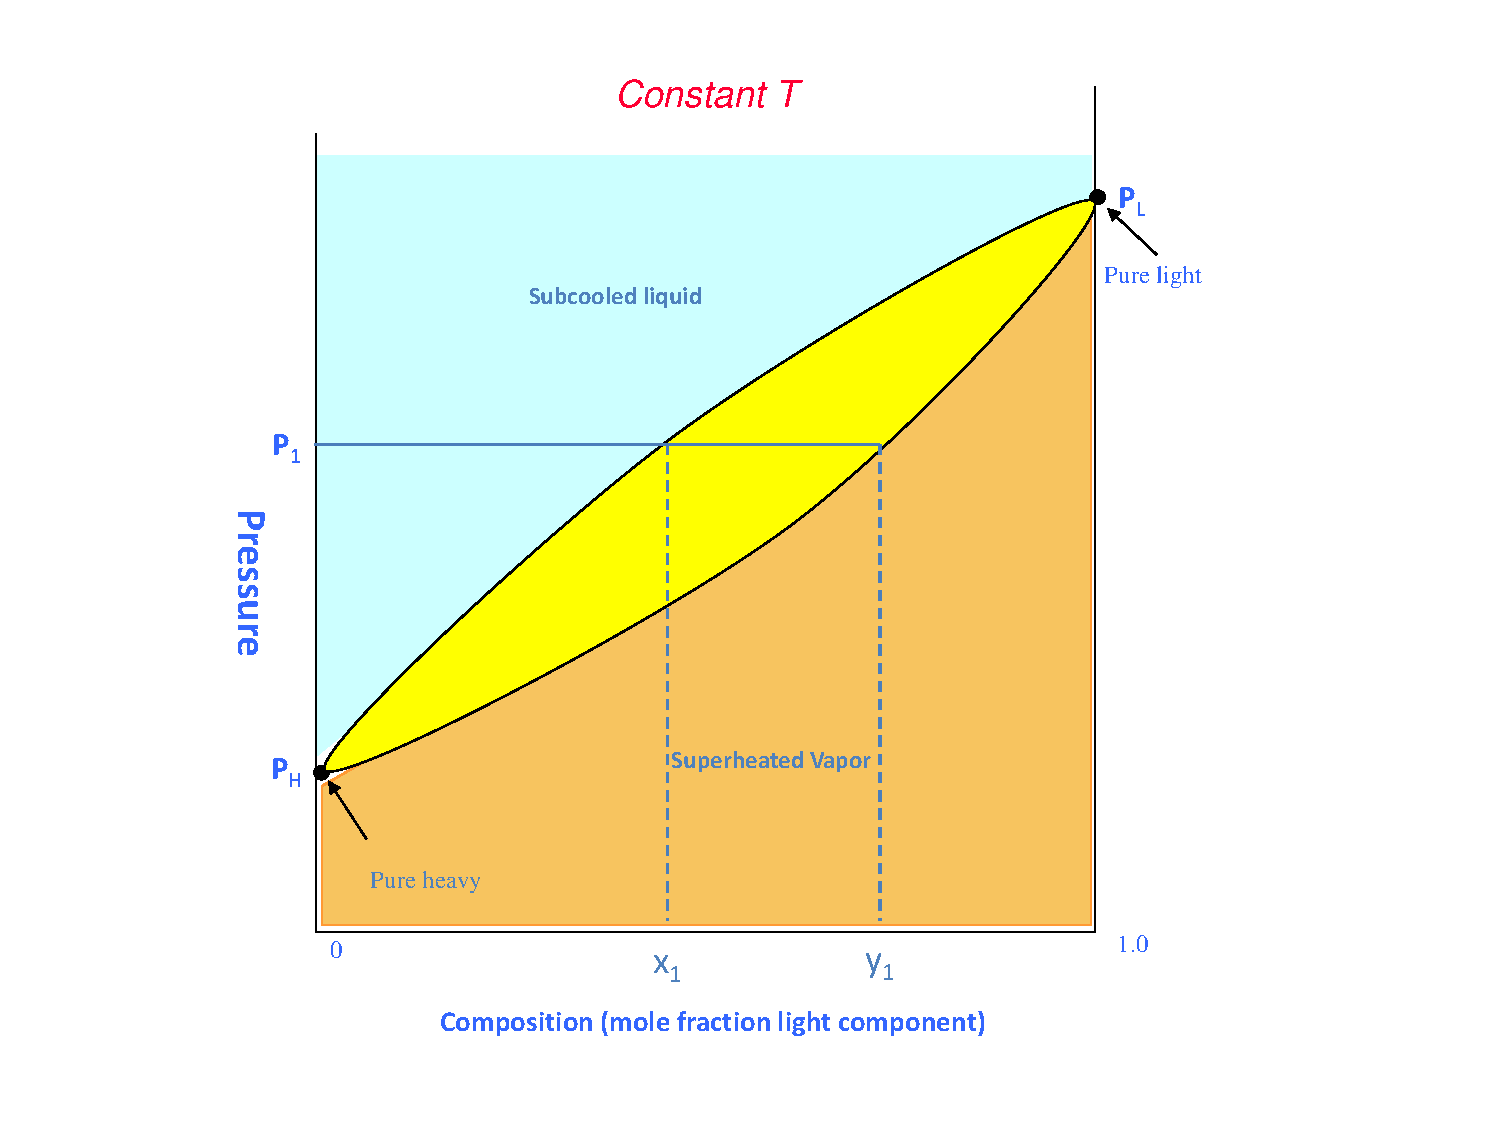
\includegraphics[width=.5\linewidth,clip]{./../Pics/VLE_Pxy_Diagram2}}
          \vspace{-0.5cm}
          \hbox{\hspace{3.5cm}(a)\hspace{6cm}(b)}
          \vspace{-0.cm}
          \hbox{\hspace{3.cm}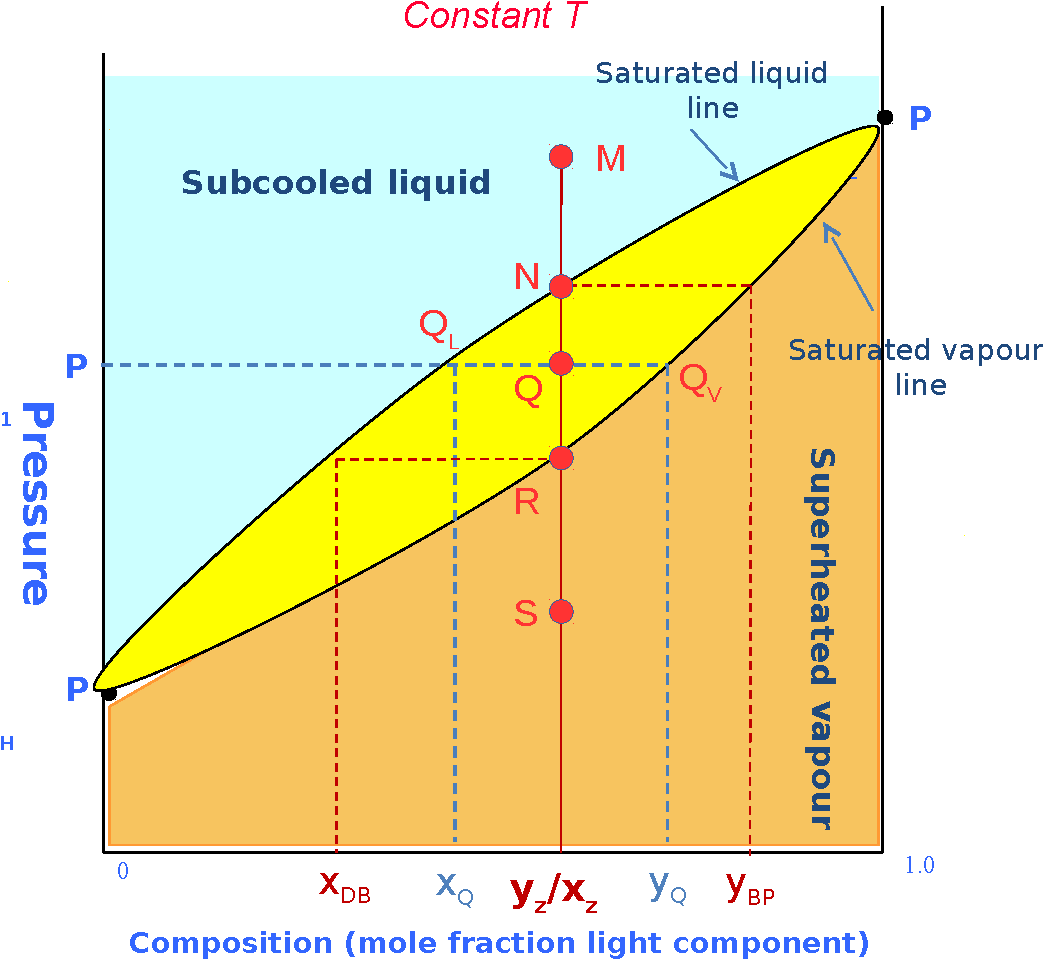
\includegraphics[width=.5\linewidth,clip]{./../Pics/VLE_Pxy_Diagram3b}}
          \vspace{-.1cm}
          \hbox{\hspace{6.8cm}(c)}}
        \vspace{-.1cm}\caption{VLE for binary mixtures: $P-xy$ diagrams at constant temperature.}\label{Chapter:VLE:Fig:Fig03}
      \end{figure}

The $x_{1},y_{1}$ axis is limited to \blue{zero} and \blue{one}, thus at $x_{1}$ (or $y_{1}$) equal to zero, $x_{2}$ (or $y_{2}$) is equal to unity, \ie there is just pure component \blue{2} in solution. Similarly at $x_{1}$ (or $y_{1}$) equal to one, $x_{2}$ (or $y_{2}$) is equal to zero, \ie there is just pure component \blue{1} in solution. The diagram also depicts points \blue{$C_{1}$} and \blue{$C_{2}$} along the vertical planes of $x_{1},y_{1}=0$ and $x_{1},y_{1}=1$, respectively. These two points are the coordinates of the critical conditions $\left(P_{c,1}, P_{c,2}, T_{c,1} \text{ and } T_{c,2}\right)$ of both \underline{pure components}. Critical coordinates for mixtures at various compositions of \blue{1} and \blue{2} lie along a line on the rounded edge of the surface between \blue{$C_{1}$} and \blue{$C_{2}$}.

For each constant temperature plane (vertical), the upper line of the solid (grey) projection is the \blue{saturated liquid line} whilst the lower line is the \blue{saturated vapour line} (the reader should remember that these lines are also present for pure substances in the $Ts$ and $Ph$ diagrams, Fig.~\ref{Chapter:ThermodynamicPropertiesPureFluids:Fig:Fig02}).

Compositions of each phase can be obtained from a parallel line linking $x_{1}$ and $y_{1}$. For example, in the `lens' \blue{U-M-R-N-U} contained in the plane \blue{0-U-M-R-1-Q-0}, the vapour phase (with composition \red{$y_{1}=\alpha$}  at $\left.\blue{K_{1}}\right)$ is in equilibrium with the liquid phase $\left(\text{with composition }\red{x_{1}=\beta}\text{ at } \blue{K_{2}}\right)$. This parallel line, \blue{$K_{1}-K_{2}$}, is called \underline{tie-line} (Fig.~\ref{Chapter:VLE:Fig:Fig03}b). The intersection of the tie-line with the saturated liquid line is referred as \blue{bubble pressure}, and the intersection with the saturated vapour line is called \blue{dew pressure} (at constant temperature).
%%% FIGURE
     \begin{figure}[h]
        \vbox{\hbox{\hspace{3.cm}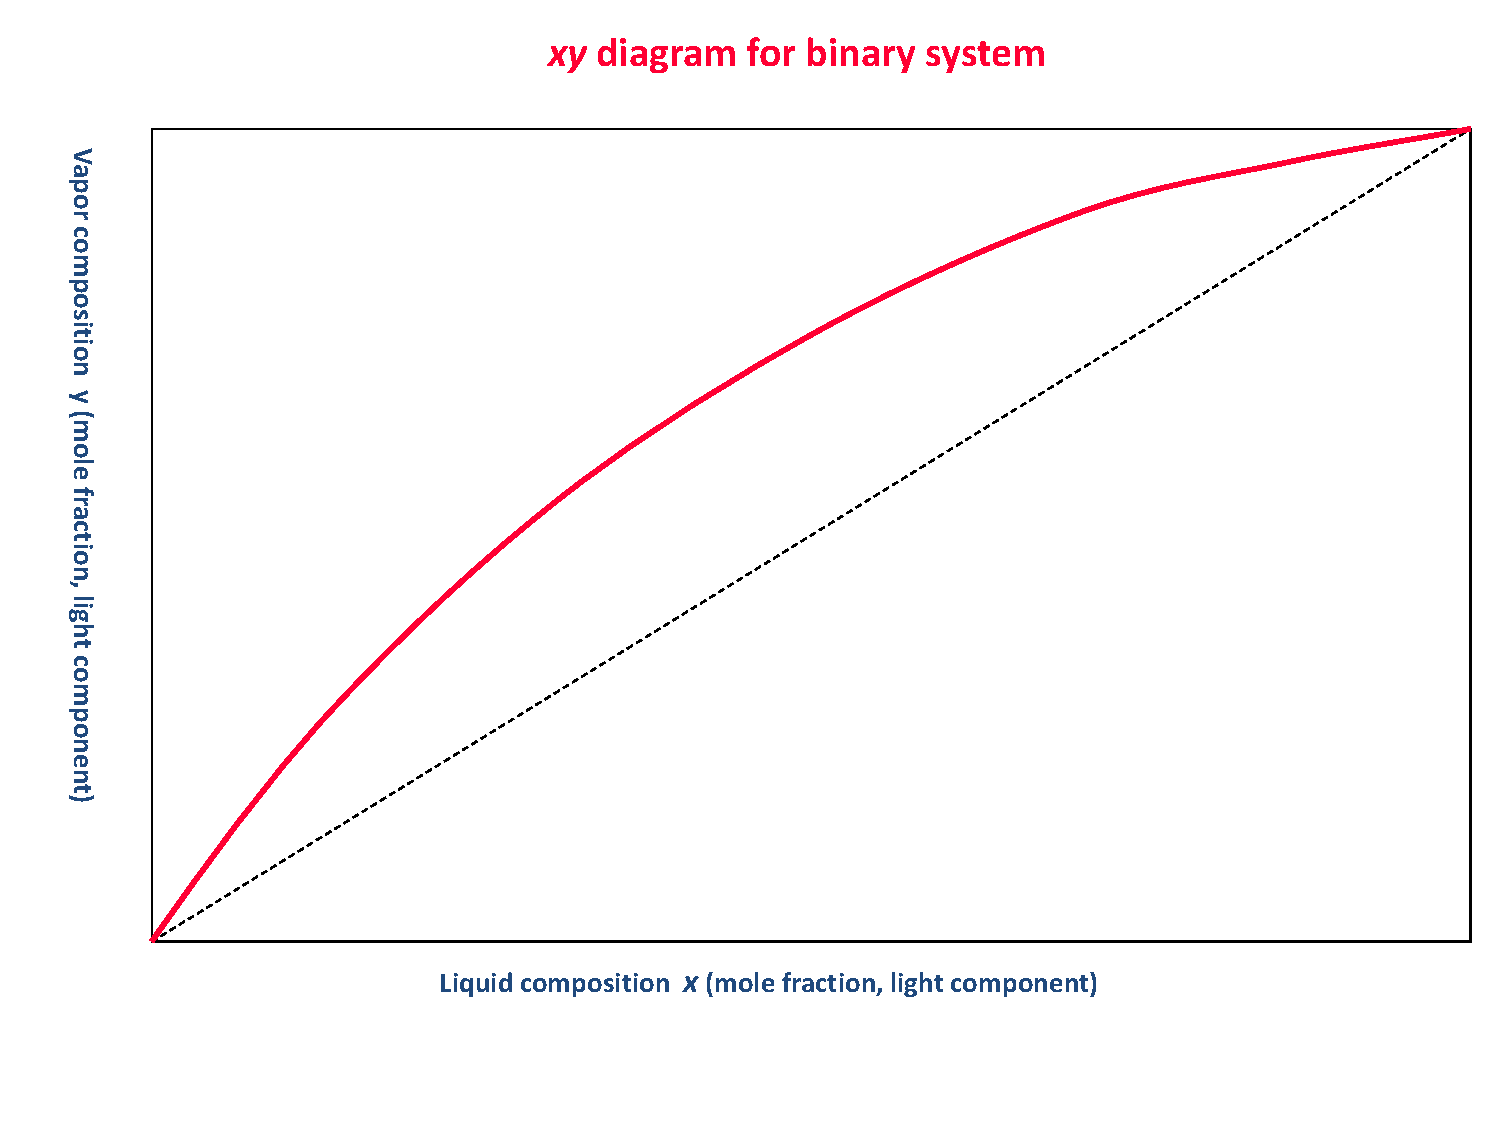
\includegraphics[width=.6\linewidth,clip]{./../Pics/VLE_xy_DiagramIdeal}}
          \vspace{-.5cm}
          \hbox{\hspace{8.cm}(a)}
          \hbox{\hspace{-1.cm}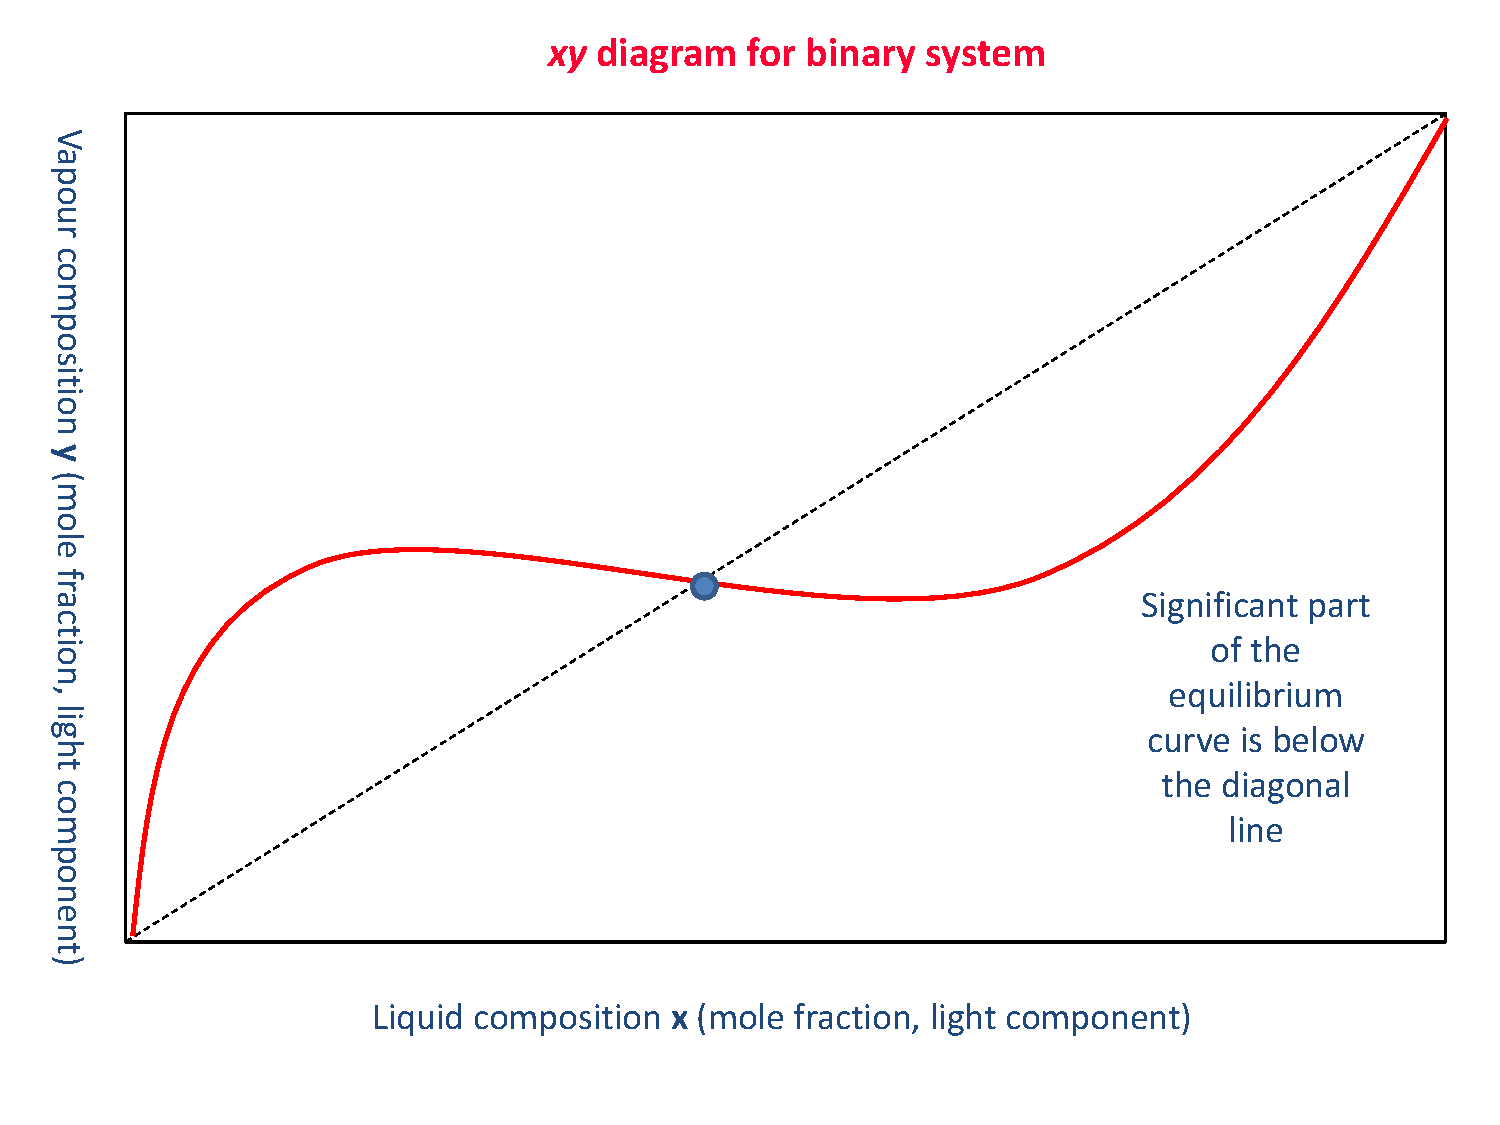
\includegraphics[width=.5\linewidth,clip]{./../Pics/VLE_xy_DiagramNonIdeal1}
            \hspace{-0.cm}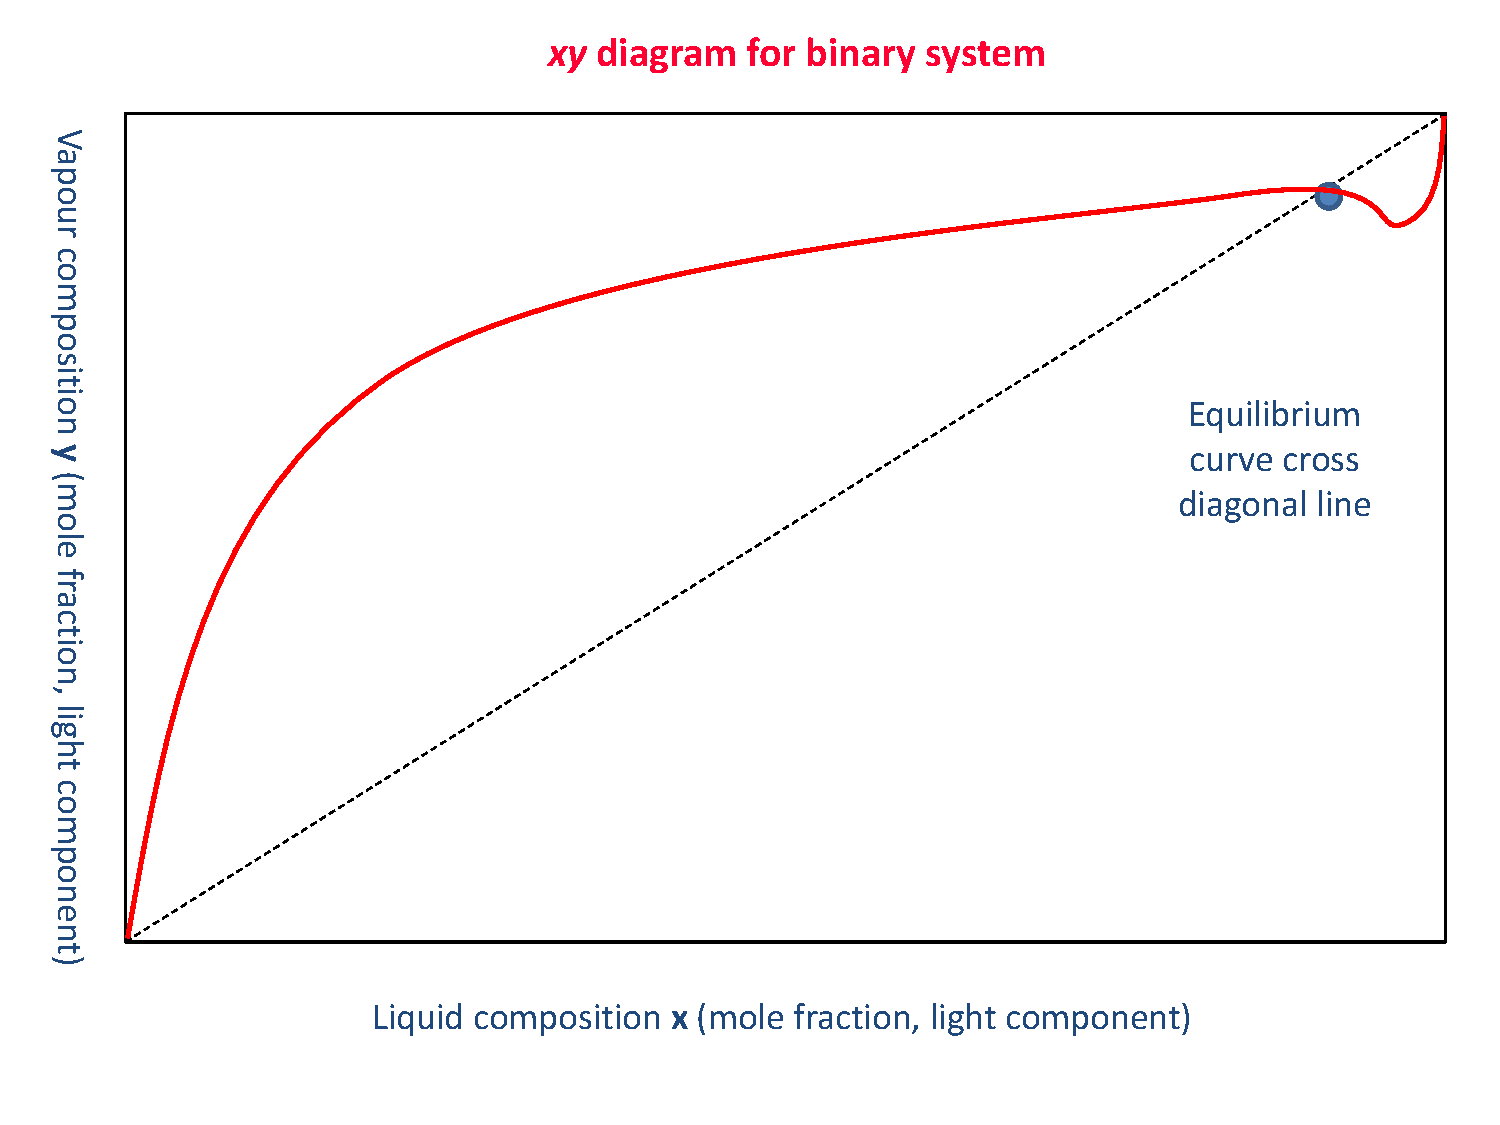
\includegraphics[width=.5\linewidth,clip]{./../Pics/VLE_xy_DiagramNonIdeal2}}
          \vspace{-.5cm}
          \hbox{\hspace{3.5cm}(b)\hspace{7.5cm}(c)}}
          \vspace{-.1cm}\caption{VLE for binary mixtures: $xy$ diagrams at constant pressure of (a) ideal and (b-c) non-ideal solutions.}\label{Chapter:VLE:Fig:Fig04}
      \end{figure}

$P-T-xy$ diagram, although insightful, is not very practical. Projections of $P-xy$ plane at constant temperature are shown in Fig.~\ref{Chapter:VLE:Fig:Fig03}. Now, let's assume that the fluid of Fig.~\ref{Chapter:VLE:Fig:Fig03}(c) is at liquid phase at coordinate \blue{$M$} with composition \blue{$\left(x_{1}=x_{z};y_{1}=0\right)$}. As pressure is reduced along the \blue{$M-S$} line, the first bubble of vapour appears at \blue{$N$}; composition at this coordinate is \blue{$\left(x_{1}=x_{z};y_{1}=y_{BP}\right)$}, and this is called \blue{\it bubble point}. Further reduction of pressure to coordinate \blue{$Q$} (still at constant temperature), the fluid becomes partially vaporised and the composition at this coordinate is given by the {\it tie-line} \blue{$Q_{L}-Q_{V}$} -- \blue{$\left(x_{1}=x_{Q};,y_{1}=y_{Q}\right)$}. \index{Bubble point}

As the pressure is continuously reduced along line \blue{$Q-R$}, more liquid is vaporised until \blue{$R$}, when the last droplet of liquid (dew) is vaporised. This coordinate is called \blue{\it dew point}. The composition at $N$ is \blue{$\left(x_{1}=x_{DB};y_{1}=y_{z}\right)$}. Continued reduction of pressure towards \blue{$S$} leads to (pure) vapour region with composition \blue{$\left(x_{1}=0,y_{1}=y_{z}\right)$}.\index{Dew point}

     Another common phase diagram is the $x-y$, Fig.~\ref{Chapter:VLE:Fig:Fig04}(a), in which either pressure or temperature is kept constant. In this diagram, at constant pressure, there are two curves, the upper curve represents the composition at equilibrium with varying temperature. The straight line represents the equimolar composition, \ie $x_{1}=y_{1}$. However, in several solutions of industrial interest, molecular attractive forces from the heavier component (2) keep molecules of the more volatile component in the liquid solution, constraining its evaporation. This leads into an equilibrium pressure smaller than the expected at the same liquid composition. Such deviation from ideality is called \blue{\it azeotropy}. In practical terms, any component from solutions can often be separated through distillation processes, however azeotropes may lead to vapour-liquid-liquid equilibrium (VLLE) and other separations strategies may need to be used.\index{Azeotropy}
     
%%% SUBSECTION
\subsection{VLE Models: Raoult's Law}\label{Chapter:VLE:Section:RaoultsLaw}
  \begin{subequations}
      The diagrams of binary (as well as multi-component) mixtures shown in the previous section are obtained from experiments and introduce a qualitative analysis of the PVT behaviour of solutions. However, classic thermodynamics provides a mathematical framework for systematic correlation, extension, generalisation and interpretation of data.\index{Raoult's law|see {Solutions}}\index{Solutions!Raoult's law}
      \begin{shaded}
        For ideal vapour-liquid systems, the \blue{Raoult's law} provides a relation between the compositions of the vapour and liquid phases,
           \begin{equation}
             P_{i} = y_{i}P = x_{i}P_{i}^{\text{sat}},\;\;\;\forall i\in\left\{1,2,\cdots,\mathcal{C}\right\},\label{Chapter:VLE:Eqn:RaoultLaw} 
           \end{equation}
      \end{shaded}
      where $P_{i}$ is known as  partial pressure (Eqn.~\ref{Chapter:Intro_Property_of_Gases:Eqn:PartialPressure_1}) and $P_{i}^{\text{sat}}$ is the saturated pressure (or saturated vapour pressure) of pure species $i$ and was defined in Section~\ref{Chapter:ThermodynamicPropertiesPureFluids:Section:ClapeyronRelations}. This rather simple relation can only be applied to ideal solutions (for both phases). For a gas mixture to be considered ideal the pressure need to be equal or smaller than atmospheric. There are several relations for ideal gas mixtures, \eg\index{Pressure!Partial}
       \begin{enumerate}[a)]
               \item Dalton's Law (Section~\ref{Chapter:Intro_Property_of_Gases:Section:MixtureGases}):\index{Gases!Dalton's law}
                  \begin{equation}
                      P = \summation[P_{i}]{i=1}{\mathcal{C}} = \summation[y_{i}P]{i=1}{\mathcal{C}}\label{Chapter:VLE:Eqn:PartialMolarProperties:DaltonLaw}
                  \end{equation}
           \item Amagat's Law:\index{Gases!Amagat's law}\index{Amagat's law|see {Gases}}
              \begin{equation}
                  V^{\text{t}} = \summation[V_{i}]{i=1}{\mathcal{C}} = \summation[y_{i}V^{\text{t}}]{i=1}{\mathcal{C}}\label{Chapter:VLE:Eqn:PartialMolarProperties:AmagatLaw}
              \end{equation}
           \item Kay's rule for pseudo-critical temperature and pressure:\index{Gases!Kay's law}\index{Kay's law|see {Gases}}
              \begin{equation}
                  T_{c}^{\text{t}} = \summation[y_{i}T_{c,i}]{i=1}{\mathcal{C}},\;\;\text{ and }\;\;P_{c}^{\text{t}} = \summation[y_{i}P_{c,i}]{i=1}{\mathcal{C}}\label{Chapter:VLE:Eqn:PartialMolarProperties:KayLaw}
              \end{equation}
       \end{enumerate}
       Liquid solutions are considered ideals if the molecular interaction between the similar species is identical to that between dissimilar species. Thermodynamics of liquid solutions are the main focus of Chapter~\ref{Chapter:SolutionThermodynamics}.
       
  \end{subequations}

  \medskip
   % Example
   \begin{MyExample}{\begin{center}{\bf Example}\end{center}}
     \begin{example}\label{Chapter:VLE:Example1}
       Assuming a mixture of n-pentane $\left(nC_{5}\right)$ and n-heptane $\left(nC_{7}\right)$ is ideal, draw vapour-liquid $x_{5}\times y_{5}$ and $P-x_{5}y_{5}$ equilibrium diagrams for this mixtures at constant temperature of 50$^{\circ}$C. Given $P^{\text{sat}}$ relation,
       \begin{displaymath}
         \ln{P_{i}^{\text{sat}}} = A_{i} - \frc{B_{i}}{RT}
       \end{displaymath}
       with $A_{nC_{5}}=10.422$, $A_{nC_{7}}=11.431$, $B_{nC_{5}}=26799 \text{ J.mol}^{-1}$ and $B_{nC_{7}}=35200 \text{ J.mol}^{-1}$. Also [$P$] = bar and [$T$] = K.
     \end{example}

% SOLUTION
     \noindent{\bf Solution:}
        At $T=$50$^{\circ}$C = 323.15 K, vapour saturated pressures for $nC_{5}$ and $nC_{7}$ (for short notation, let's use 5 and 7 as $nC_{5}$ and $nC_{7}$, respectively) are
           \begin{displaymath}
              P_{5}^{\text{sat}} = 1.5639\text{ bar}\;\;\text{ and }\;\;P_{7}^{\text{sat}} = 0.1881\text{ bar}.
           \end{displaymath}
           In order to calculate the equilibrium pressure at each liquid $nC_{5}$ composition, $x_{5}$,
           \begin{eqnarray}
               && P_{i} = x_{i}P_{i}^{\text{sat}} \;\;\Longleftrightarrow \;\; P = \summation[P_{i}]{i=1}{\mathcal{C}} = \summation[x_{i}P_{i}^{\text{sat}}]{i=1}{\mathcal{C}} \nonumber \\
               && P = x_{5}P_{5}^{\text{sat}} + x_{7}P_{7}^{\text{sat}} = x_{5}P_{5}^{\text{sat}} + \left(1-x_{5}\right)P_{7}^{\text{sat}} \nonumber 
           \end{eqnarray}
           And for vapour composition (Raoult's law),
           \begin{displaymath}
               y_{i} P = x_{i}P_{i}^{\text{sat}}  \;\;\Longleftrightarrow \;\; y_{5} = \frc{x_{5}P_{5}^{\text{sat}}}{P},
           \end{displaymath}
           replacing pressure, $P$, from the previous equation
           \begin{displaymath}
               y_{5} = \frc{x_{5}P_{5}^{\text{sat}}}{x_{5}P_{5}^{\text{sat}} + \left(1-x_{5}\right)P_{7}^{\text{sat}}}.
           \end{displaymath}
           The $x_{5} \times y_{5}$ diagram may be plot by giving values to $0.0\leq x_{5} \leq 1.0$ and calculating $x_{5}$ through the equation above.

           The $P-x_{5}y_{5}$ diagram may be plot using the relations,
           \begin{displaymath}
               y_{5} = \frc{x_{5}P_{5}^{\text{sat}}}{P}\;\;\;\text{ and }\;\;\; P = x_{5}P_{5}^{\text{sat}} + \left(1-x_{5}\right)P_{7}^{\text{sat}} \;\Longrightarrow\; x_{5} = \frc{P-P_{7}^{\text{sat}}}{P_{5}^{\text{sat}}-P_{7}^{\text{sat}}}.
           \end{displaymath}
           Thus, given values for $P_{7}^{\text{sat}}\leq P \leq P_{5}^{\text{sat}}$ $\Rightarrow$ Calculate $x_{5}$  $\Rightarrow$ Calculate $y_{5}$.
           \bigskip
           
           \hbox{
             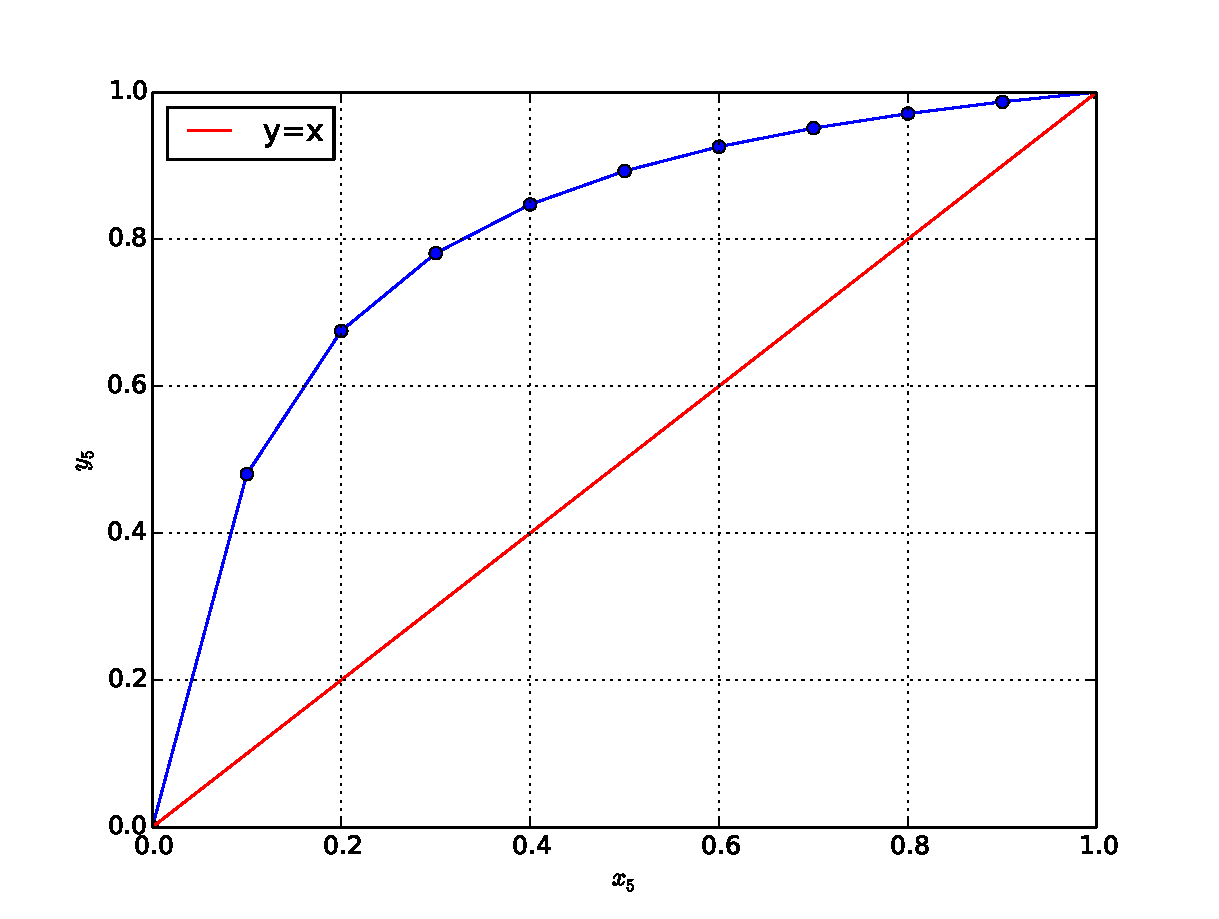
\includegraphics[width=.5\linewidth,clip]{./Figs/Mod4Ex1}
             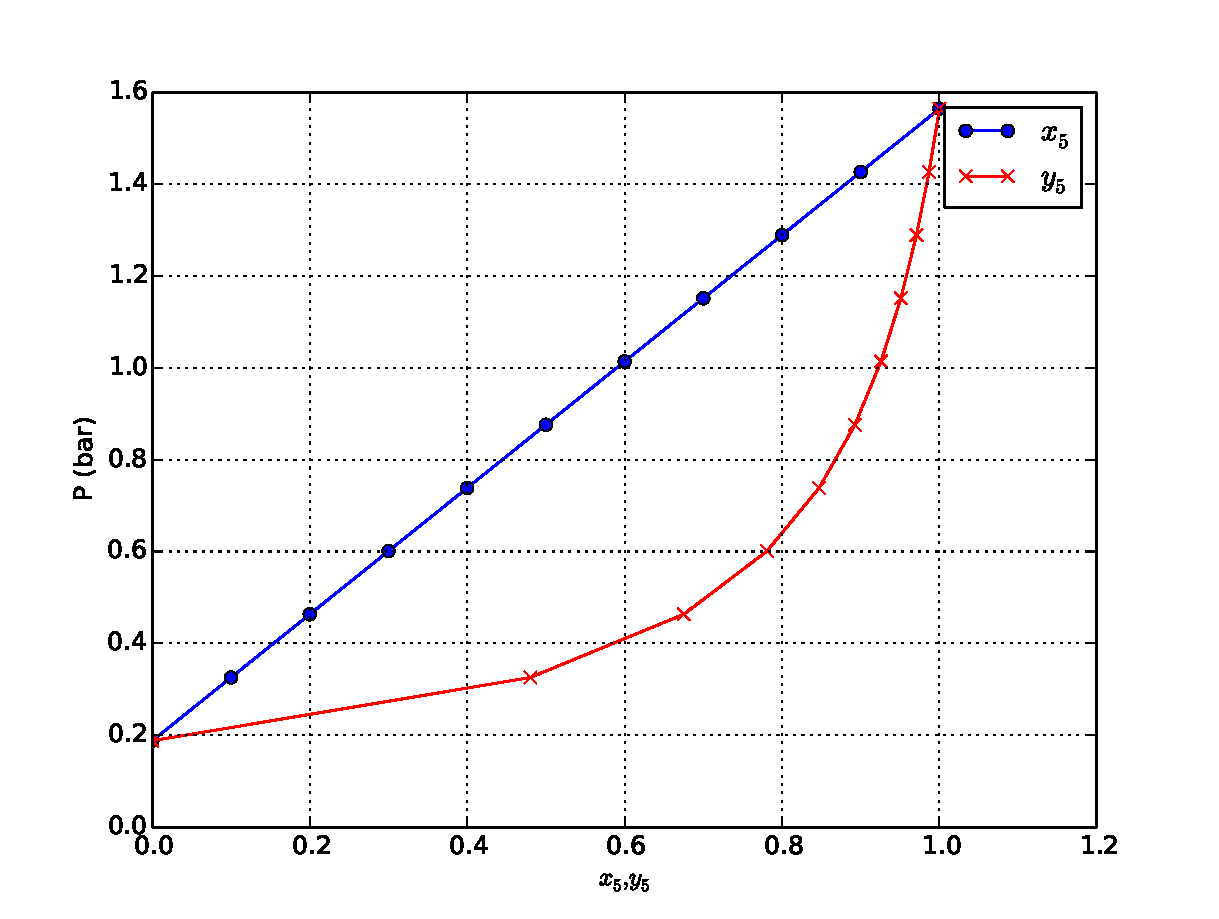
\includegraphics[width=.5\linewidth,clip]{./Figs/Mod4Ex1b}}
           
   \end{MyExample} 

  \medskip
   % Example
   \begin{MyExample}{\begin{center}{\bf Example}\end{center}}
     \begin{example}\label{Chapter:VLE:Example2}
       Assuming a mixture of n-pentane $\left(nC_{5}\right)$ and n-heptane $\left(nC_{7}\right)$ is ideal, draw vapour-liquid $x_{5}\times y_{5}$ and $T-x_{5}y_{5}$ equilibrium diagrams for this mixtures at constant pressure of 1.013 bar. Given $P^{\text{sat}}$ relation,
    \begin{displaymath}
      \ln{P_{i}^{\text{sat}}} = A_{i} - \frc{B_{i}}{RT}
    \end{displaymath}
    with $A_{nC_{5}}=10.422$, $A_{nC_{7}}=11.431$, $B_{nC_{5}}=26799 \text{ J.mol}^{-1}$ and $B_{nC_{7}}=35200 \text{ J.mol}^{-1}$. Also [$P$] = bar and [$T$] = K.
     \end{example}

% SOLUTION
     \noindent{\bf Solution:}
     In this problem, equilibrium temperature and compositions are not known, thus
          \begin{displaymath}
              P = x_{5}P_{5}^{\text{sat}} + x_{7}P_{7}^{\text{sat}} = x_{5}P_{5}^{\text{sat}} + \left(1 - x_{5}\right)P_{7}^{\text{sat}} = 1.013\text{ bar},
          \end{displaymath}
          where $P_{i}^{\text{sat}}$ is non-linear function of the temperature $T$, \ie
          \begin{displaymath}
              P = x_{5}\exp{\left(A_{5} - \frc{B_{5}}{RT}\right)} + \left(1 - x_{5}\right)\exp{\left(A_{7} - \frc{B_{7}}{RT}\right)}.
          \end{displaymath}
          This equation has 2 unknowns, $x_{5}$ and $T$, however we know that $0.0\leq x_{5} \leq 1.0$, thus we can give values on this range $\Rightarrow$ calculate $T$  $\Rightarrow$  obtain $y_{5}$.
          \begin{center}
              \begin{tabular}{ c c c | c c c}
                  $\mathbf{x_{5}}$ & $\mathbf{T}${\bf(K)}  & $\mathbf{y_{5}}$ & $\mathbf{x_{5}}$ & $\mathbf{T}${\bf(K)}  & $\mathbf{y_{5}}$ \\
                    0.0000          & 370.80                & 0.0000         & 0.6000          & 323.13                & 0.9257          \\
                    0.1000          & 357.80                & 0.4050         & 0.7000          & 319.12                & 0.9528          \\
                    0.2000          & 347.73                & 0.6249         & 0.8000          & 315.60                & 0.9728          \\
                    0.3000          & 339.73                & 0.7535         & 0.9000          & 312.47                & 0.9881          \\
                    0.4000          & 333.21                & 0.8345         & 1.0000          & 309.67                & 1.0000          \\
                    0.5000          & 327.77                & 0.8881         &                 &                       &                 
              \end{tabular}
           \end{center}
           \medskip
             \hbox{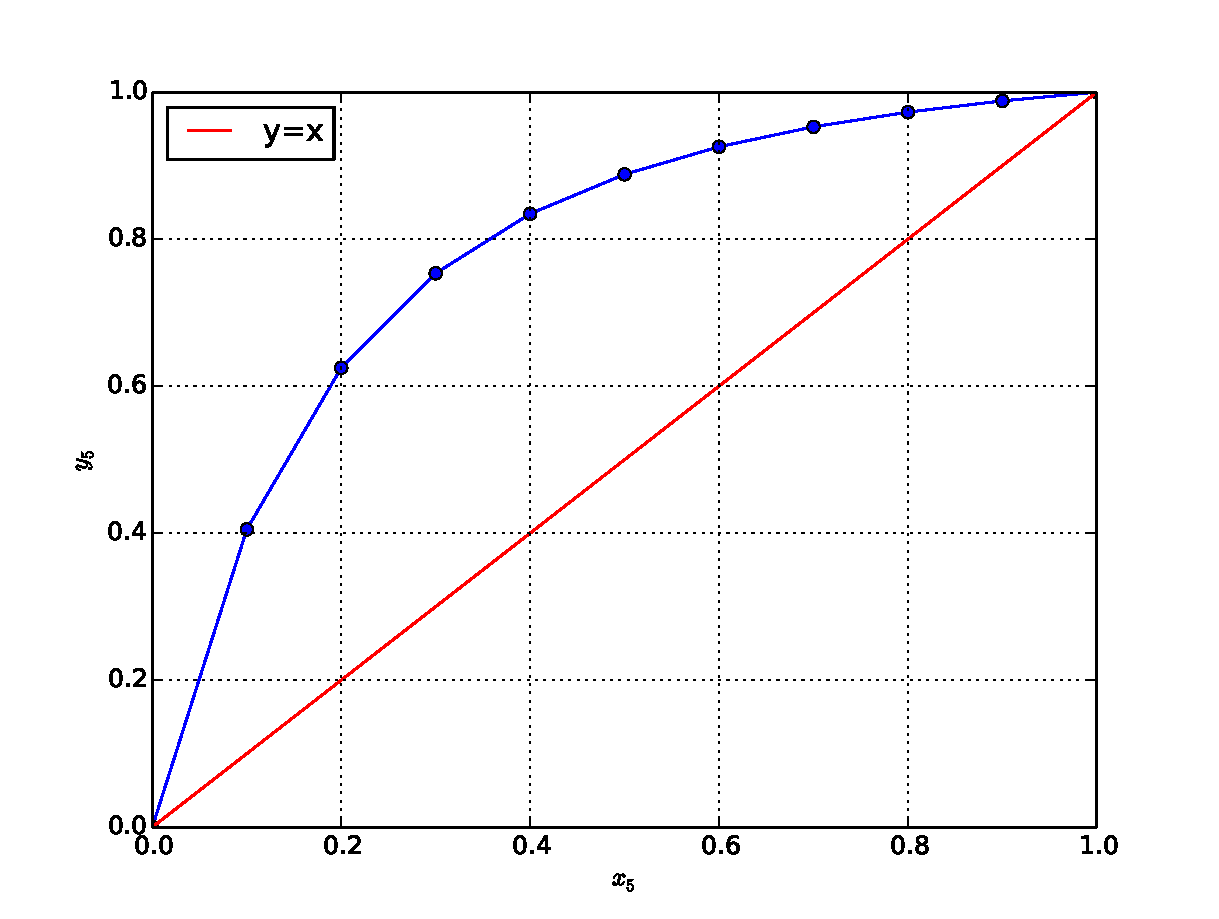
\includegraphics[width=.5\linewidth,clip]{./Figs/Mod4Ex2a}
                   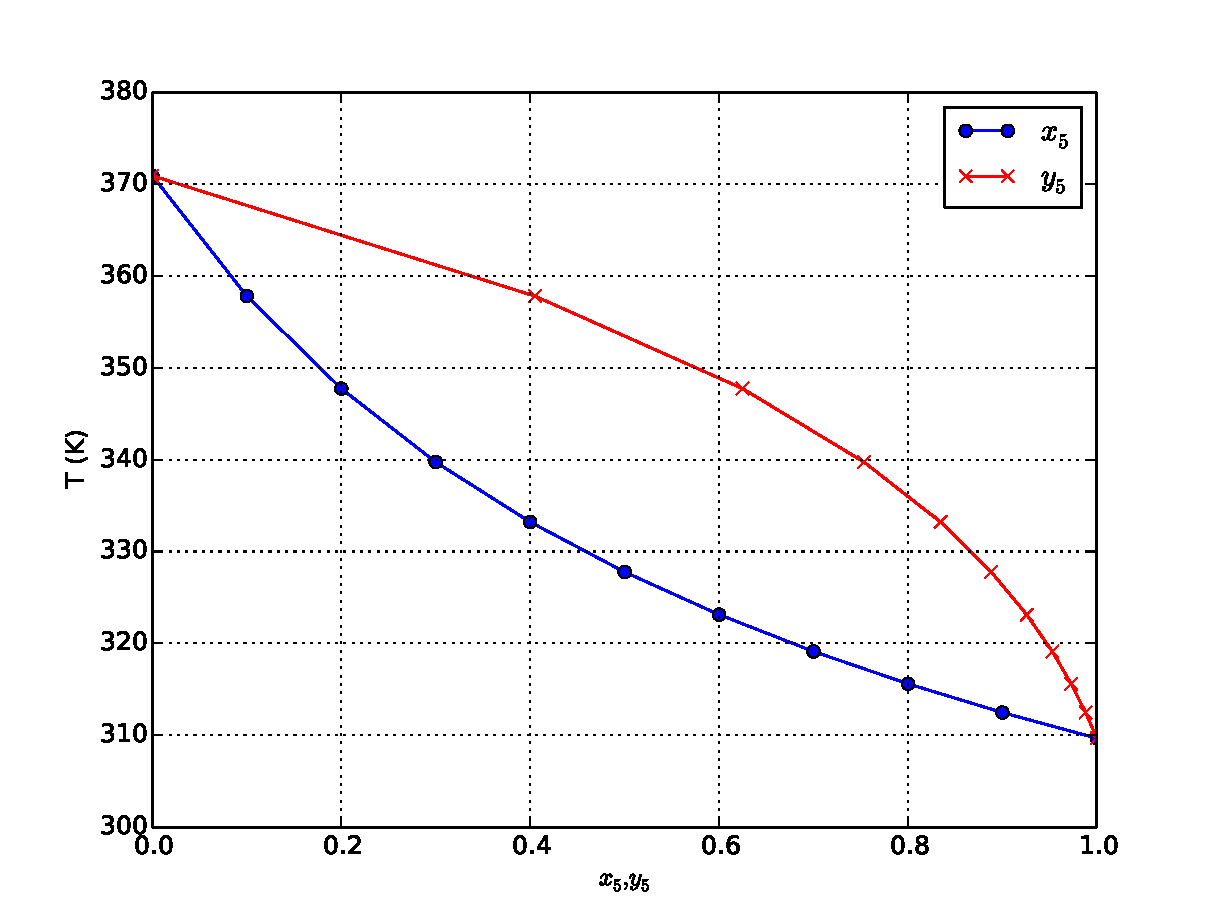
\includegraphics[width=.5\linewidth,clip]{./Figs/Mod4Ex2b}}
             
   \end{MyExample}

%%% SUBSECTION
\subsection{VLE Models: Henry's Law}\label{Chapter:VLE:Section:HenryLaw}\index{Henry's law|see {Solutions}}\index{Solutions!Henry's law}
A typical application of VLE is when gases are solubilised in liquid solutions, \eg O$_{2}$ in water, CO$_{2}$ in soft drinks, air in the blood stream etc. In these cases, gases have relatively low solubility (mole fraction varying between 10$^{-5}$ to 10$^{-2}$) in liquid solvents. In ideal solutions, both the more volatile (\ie solute) and the less volatile (\ie solvent) follow the Raoult’s law. However, for real solutions at low concentrations, although the vapour pressure $\left(P^{\text{sat}}\right)$ of the solute is proportional to its mole fraction, the constant of proportionality is not the vapour pressure of the pure substance. For such cases, a new relation is required that relates compositions in both phases and the pressure,
\begin{shaded}
  \begin{equation}
      P_{i} = y_{i}P = x_{i}\mathcal{H}_{i},\label{Chapter:VLE:Eqn:HenryLaw} 
  \end{equation}
\end{shaded}
\noindent where $\mathcal{H}$ is the Henry's constant obtained experimentally. Values of Henty's contant for several gases dissolved in water at 25$^{\circ}$C is shown in Table~\ref{Chapter:VLE:Table:HenryLawTable}
%%% TABLE
 \begin{table}
  \begin{center}
    \begin{tabular}{l r || l r }
      \hline
       {\bf Gas}    &  ${\bf \mathcal{H}\text{ (bar)}}$ & {\bf Gas}    &  ${\bf \mathcal{H}\text{ (bar)}}$ \\
      \hline
         Acetylene  &   1350                            & He           &  126600 \\
         Air        &   72950                           & H$_{2}$      &  71600  \\
         CO$_{2}$    & 1670                              & H$_{2}$S     & 550 \\
         CO         &  54600                            &  CH$_{4}$    &  41850 \\
         C$_{2}$H$_{6}$ & 30600                          &  N$_{2}$     & 87650  \\
         Ethylene  & 11550                              & O$_{2}$      & 44380 \\
      \hline
    \end{tabular}
    \caption{Henry's constant for gases dissolved in water at 25$^{\circ}$C.}\label{Chapter:VLE:Table:HenryLawTable}
  \end{center}
\end{table}

%%% SUBSECTION
\subsection{VLE Models: K-Value Correlations for Hydrocarbon Systems}\label{Chapter:VLE:Section:K_Values}\index{K-Value|see {Solutions}}\index{Solutions!K-Values}
As discussed in Section~\ref{Chapter:VolumetricPropertiesPureSubstances:Section:CubicEOS}, cubic equations of state are often used to describe the PVT behaviour of vapour and liquid phases of pure chemical species and mixtures. Although the use of cubic EOS is widely spread over the chemical industry, applicability to liquid phase is still limited. Several alternatives have been proposed and developed over the past 50 years, one of them, mostly used in petroleum and petrochemical industry for hydrocarbons, is called {\it K-value correlation}. $K$ is defined as
\begin{shaded}
   \begin{equation}
      K_{i} = \frc{P_{i}^{\text{sat}}}{P} = \frc{y_{i}}{x_{i}}.\label{Chapter:VLE:Eqn:KValue}
   \end{equation}
\end{shaded}
Values for $K_{i}$ are tabulated for a large number of hydrocarbons at several pressure and temperature conditions and can be found in any chemical engineering handbook as part of \blue{DePriester chart} (Fig.~\ref{Chapter:VLE:Fig:Fig05}).\index{DePriester chart|see {Solutions}}\index{Solutions!DePriester chart}
%%% FIGURE
  \begin{figure}[h]
     \begin{center}
         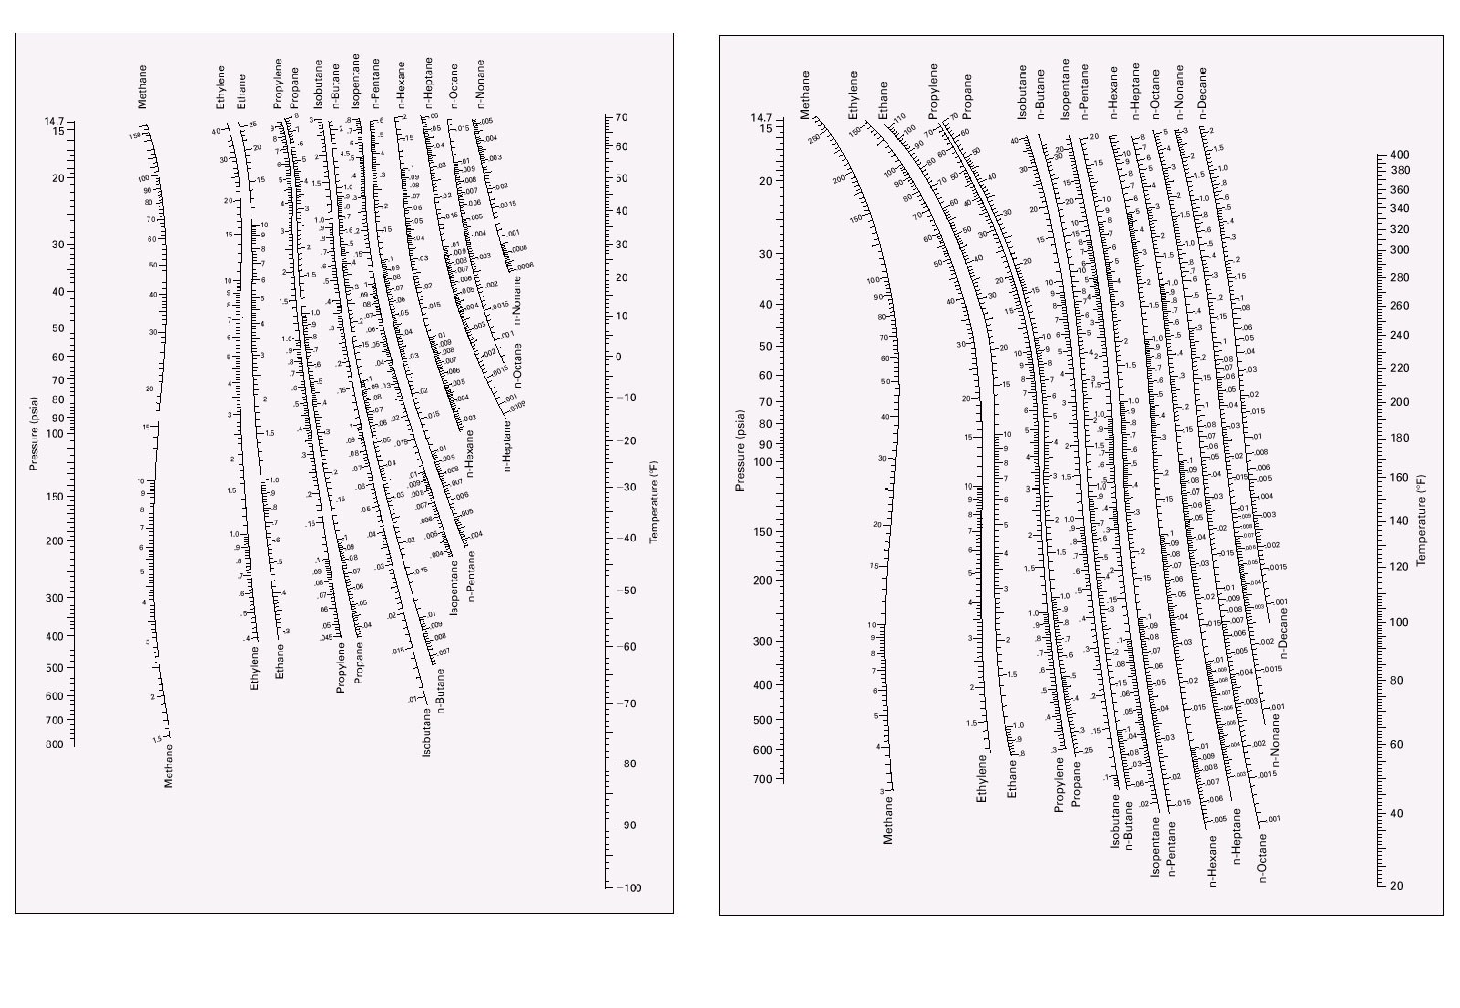
\includegraphics[width=1.\linewidth,clip]{./Figs/DePriesterCharts}
     \end{center}
     \caption{DePriester chart for several hydrocarbons \citep[extracted from][]{SmithVanNess_Book}.}\label{Chapter:VLE:Fig:Fig05}
  \end{figure}
  
%%% SECTION
  \section{Industrial Applications: Multi-Component VLE}\label{Chapter:VLE:Section:IndApplications}
  
%%% SUBSECTION
\subsection{Dew-point and Bubble-point Calculations using Raoult’s Law }\label{Chapter:VLE:Section:DewBubblePoint}\index{Bubble point}\index{Dew point}
Let's consider a vapour-liquid system containing $\mathcal{C}$ chemical species. From the phase rule the number of degrees of freedom is $\mathcal{C}$, that may be $T$, $P$, $x_{i}$ and/or $y_{i}$. Four types of problems are possible:
\begin{center}
   \begin{tabular}{|l c c|}
      \hline 
      $\mathbf{VLE}$ {\bf Problem} & {\bf Specified Variables} &  {\bf Computed Variables} \\  
      \hline
          {\bf Bubble Pressure}        &  $T$ and $x_{i}$           &   $P$ and $y_{i}$          \\
          {\bf Dew Pressure}           &  $T$ and $y_{i}$           &   $P$ and $x_{i}$          \\
          {\bf Bubble Temperature}     &  $P$ and $x_{i}$           &   $T$ and $y_{i}$          \\
          {\bf Dew Temperature}        &  $P$ and $y_{i}$           &   $T$ and $x_{i}$          \\     
      \hline
   \end{tabular}
\end{center}
Such problems are calculated using three relations:
\begin{displaymath}
    P_{i} = y_{i}P = x_{i}P_{i}^{\text{sat}}, \;\;\; \summation[x_{i}]{i=1}{\mathcal{C}} = 1, \;\;\text{ and }\;\; \summation[y_{i}]{i=1}{\mathcal{C}} = 1,
\end{displaymath}
bearing in mind that $P_{i}^{\text{sat}}$ is expressed as a function of $T$. Thus,
\begin{enumerate}[a)]
    \item Bubble pressure: Given $T$ and $x_{i}$ $\left(\text{with }i=1,\cdots,\mathcal{C}\right)$, find $P$ that solves,
        \begin{displaymath}
           \summation[y_{i}]{i=1}{\mathcal{C}} = 1 \;\;\Longrightarrow\;\; \summation[\frc{x_{i}P_{i}^{\text{sat}}}{P}]{i=1}{\mathcal{C}} = 1,
        \end{displaymath}
        and then calculate $y_{i}= \frc{x_{i}P_{i}^{\text{sat}}}{P}$.
        
    \item Bubble temperature: Given $P$ and $x_{i}$ $\left(\text{with }i=1,\cdots,\mathcal{C}\right)$, find $T$ that solves,
        \begin{displaymath}
           \summation[y_{i}]{i=1}{\mathcal{C}} = 1 \;\;\Longrightarrow\;\; \summation[\frc{x_{i}P_{i}^{\text{sat}}}{P}]{i=1}{\mathcal{C}} = 1,
        \end{displaymath}
        and then calculate $y_{i}= \frc{x_{i}P_{i}^{\text{sat}}}{P}$.
      
    \item Dew pressure: Given $T$ and $y_{i}$ $\left(\text{with }i=1,\cdots,\mathcal{C}\right)$, find $P$ that solves,
        \begin{displaymath}
           \summation[x_{i}]{i=1}{\mathcal{C}} = 1 \;\;\Longrightarrow\;\; \summation[\frc{y_{i}P}{P_{i}^{\text{sat}}}]{i=1}{\mathcal{C}} = 1,
        \end{displaymath}
        and then calculate $y_{i}= \frc{x_{i}P_{i}^{\text{sat}}}{P}$.
      
    \item Dew temperature: Given $P$ and $y_{i}$ $\left(\text{with }i=1,\cdots,\mathcal{C}\right)$, find $T$ that solves,
        \begin{displaymath}
           \summation[x_{i}]{i=1}{\mathcal{C}} = 1 \;\;\Longrightarrow\;\; \summation[\frc{y_{i}P}{P_{i}^{\text{sat}}}]{i=1}{\mathcal{C}} = 1,
        \end{displaymath}
        and then calculate $y_{i}= \frc{x_{i}P_{i}^{\text{sat}}}{P}$.
\end{enumerate}


  \medskip
   % Example
   \begin{MyExample}{\begin{center}{\bf Example}\end{center}}
     \begin{example}\label{Chapter:VLE:Example3}\citep{Sandler_Book}
       Estimate the bubble and dew point temperatures of a mixture of 25 mol-$\%$ of n-pentane, 45 mol-$\%$ of n-hexane and 30 mol-$\%$ of n-heptane at 1.013 bar. Given $P^{\text{sat}}$ relation,
    \begin{displaymath}
      \ln{P_{i}^{\text{sat}}} = A_{i} - \frc{B_{i}}{RT}
    \end{displaymath}
    with $A_{nC_{5}}=10.422$, $A_{nC_{6}}=10.456$, $A_{nC_{7}}=11.431$, $B_{nC_{5}}=26799 \text{ J.mol}^{-1}$, $B_{nC_{6}}=29676 \text{ J.mol}^{-1}$ and $B_{nC_{7}}=35200 \text{ J.mol}^{-1}$. Also [$P$] = bar and [$T$] = K.
     \end{example}

% SOLUTION
     \noindent{\bf Solution:}
     Assuming the solution is ideal and the gas phase behaves as an ideal gas (\ie low/room pressure), Raoult's law can be used,
    \begin{displaymath}
       x_{i}P_{i}^{\text{sat}} = y_{i}P = P_{i} \;\;\text{ with }\;\; \summation[x_{i}P_{i}^{\text{sat}}]{i}{} = \summation[P_{i}]{i}{} = P, \;\summation[x_{i}]{i}{}=1=\summation[y_{i}]{i}{}.
    \end{displaymath}
    For the bubble point, the procedure is:
    \begin{enumerate}[i)]
       \item choose an initial guess for the bubble point temperature, $T^{\text{guess}}$;
       \item calculate $y_{i}=\frc{x_{i}P_{i}^{\text{sat}}}{P}$;
       \item then:
           \begin{itemize}
              \item if $\summation[y_{i}]{i}{} = 1 \;\;\Rightarrow \;\; T^{\text{guess}} = T$;
              \item if $\summation[y_{i}]{i}{} > 1 \;\;\Rightarrow \;\; T^{\text{guess}} > T \;\; \Rightarrow\;\; \text{adjust } T^{\text{guess}}$;
              \item if $\summation[y_{i}]{i}{} < 1 \;\;\Rightarrow \;\; T^{\text{guess}} < T \;\; \Rightarrow\;\; \text{adjust } T^{\text{guess}}$.
           \end{itemize}
    \end{enumerate}
    Thus, for this problem,
    \begin{displaymath}
        \summation[y_{i}]{i}{} = 1\;\; \Longleftrightarrow \;\; \frc{x_{5}P_{5}^{\text{sat}}}{P} + \frc{x_{6}P_{6}^{\text{sat}}}{P} + \frc{x_{7}P_{7}^{\text{sat}}}{P} = 1,
    \end{displaymath}
    where $P_{i}^{\text{sat}}$ is a function of $T$, 
    \begin{displaymath}
        \frc{x_{5}\exp{\left(A_{5}-\frc{B_{5}}{RT}\right)}}{P} + \frc{x_{6}\exp{\left(A_{6}-\frc{B_{6}}{RT}\right)}}{P} + \frc{x_{7}\exp{\left(A_{7}-\frc{B_{7}}{RT}\right)}}{P} = 1
    \end{displaymath}
    Using $T^{\text{guess}}=298.15$ K as initial guess, $T=334.9380$ K (bubble point temperature). Now, calculating the vapour composition, $y_{i}=\frc{x_{i}P_{i}^{\text{sat}}}{P}$ leads to,
    \begin{displaymath}
        y_{5} =0.5483,\;\; y_{6} = 0.3634\;\;\text{ and }\;\;y_{7} = 0.0883\;\;\Rightarrow\;\; \summation[y_{i}]{i}{} = 1.0000
    \end{displaymath}

\medskip
    For the dew point, the procedure is:
    \begin{enumerate}[i)]
       \item choose an initial guess for the dew point temperature, $T^{\text{guess}}$;
       \item calculate $x_{i}=\frc{y_{i}P}{P_{i}^{\text{sat}}}$;
       \item then:
           \begin{itemize}
              \item if $\summation[x_{i}]{i}{} = 1 \;\;\Rightarrow \;\; T^{\text{guess}} = T$;
              \item if $\summation[x_{i}]{i}{} > 1 \;\;\Rightarrow \;\; T^{\text{guess}} < T \;\; \Rightarrow\;\; \text{adjust } T^{\text{guess}}$;
              \item if $\summation[x_{i}]{i}{} < 1 \;\;\Rightarrow \;\; T^{\text{guess}} > T \;\; \Rightarrow\;\; \text{adjust } T^{\text{guess}}$.
           \end{itemize}
    \end{enumerate}
    Thus, for this problem,
    \begin{displaymath}
        \summation[x_{i}]{i}{} = 1\;\; \Longleftrightarrow \;\; \frc{y_{5}P}{P_{5}^{\text{sat}}} + \frc{y_{6}P}{P_{6}^{\text{sat}}} + \frc{y_{7}P}{P_{7}^{\text{sat}}} = 1,
    \end{displaymath}
    where $P_{i}^{\text{sat}}$ is a function of $T$, 
    \begin{displaymath}
        \frc{y_{5}P}{\exp{\left(A_{5}-\frc{B_{5}}{RT}\right)}} + \frc{x_{6}P}{\exp{\left(A_{6}-\frc{B_{6}}{RT}\right)}} + \frc{x_{7}P}{\exp{\left(A_{7}-\frc{B_{7}}{RT}\right)}}= 1
    \end{displaymath}
    Using $T^{\text{guess}}=298.15$ K as initial guess, $T=350.5857$ K (dew point temperature). Now, calculating the liquid composition, $y_{i}=\frc{x_{i}P_{i}^{\text{sat}}}{P}$ leads to,
    \begin{displaymath}
        x_{5} =0.0742\;\; x_{6} = 0.3463\;\;\text{ and }\;\;x_{7} = 0.5795\;\;\Rightarrow\;\; \summation[x_{i}]{i}{} = 1.0000
    \end{displaymath}
   \end{MyExample}

  \medskip
   % Example
   \begin{MyExample}{\begin{center}{\bf Example}\end{center}}
     \begin{example}\label{Chapter:VLE:Example4}
       Estimate the bubble and dew point pressures of a mixture of 25 mol-$\%$ of n-pentane, 45 mol-$\%$ of n-hexane and 30 mol-$\%$ of n-heptane at 73$^{\circ}$C. Given $P^{\text{sat}}$ relation,
    \begin{displaymath}
      \ln{P_{i}^{\text{sat}}} = A_{i} - \frc{B_{i}}{RT}
    \end{displaymath}
    with $A_{nC_{5}}=10.422$, $A_{nC_{6}}=10.456$, $A_{nC_{7}}=11.431$, $B_{nC_{5}}=26799 \text{ J.mol}^{-1}$, $B_{nC_{6}}=29676 \text{ J.mol}^{-1}$ and $B_{nC_{7}}=35200 \text{ J.mol}^{-1}$. Also [$P$] = bar and [$T$] = K.
     \end{example}

% SOLUTION
     \noindent{\bf Solution:}
     For the bubble point, the mixture follows Raoult's law at 73$^{\circ}$C,
      \begin{displaymath}
          P = \summation[x_{i}P_{i}^{\text{sat}}]{i}{} = x_{5}P_{5}^{\text{sat}} + x_{6}P_{6}^{\text{sat}} + x_{7}P_{7}^{\text{sat}} = 1.413\text{ bar}
      \end{displaymath}
      This is the bubble point pressure at 346.15 K. The composition of the vapour phase is,
      \begin{displaymath}
             y_{i}=\frc{x_{i}P_{i}^{\text{sat}}}{P}
             \begin{cases}
                  y_{5} = 0.5370,\\
                  y_{6} = 0.3680,\\
                  y_{7} = 0.0950,
             \end{cases}
      \end{displaymath}
      leading to $\summation[y_{i}]{i}{} = 1.0000$.

\medskip

     For the dew point, the procedure is:
    \begin{enumerate}[i)]
       \item choose an initial guess for the dew point pressure, $P^{\text{guess}}$;
       \item calculate $x_{i}=\frc{Py_{i}}{P_{i}^{\text{sat}}}$;
       \item then:
           \begin{itemize}
              \item if $\summation[x_{i}]{i}{} = 1 \;\;\Rightarrow \;\; P^{\text{guess}} = P$;
              \item if $\summation[x_{i}]{i}{} > 1 \;\;\Rightarrow \;\; P^{\text{guess}} > P \;\; \Rightarrow\;\; \text{adjust } P^{\text{guess}}$;
              \item if $\summation[x_{i}]{i}{} < 1 \;\;\Rightarrow \;\; P^{\text{guess}} < P \;\; \Rightarrow\;\; \text{adjust } P^{\text{guess}}$.
           \end{itemize}
    \end{enumerate}
    Thus, for this problem,
    \begin{displaymath}
        \summation[x_{i}]{i}{} = 1\;\; \Longleftrightarrow \;\; \frc{y_{5}P}{P_{5}^{\text{sat}}} + \frc{y_{6}P}{P_{6}^{\text{sat}}} + \frc{y_{7}P}{P_{7}^{\text{sat}}} = 1,
    \end{displaymath}
    where $P_{i}^{\text{sat}}$ is a function of $T$ (which is known in this problem!).  Solving this equation leads to $P=0.8774$ bar (dew point pressure) with composition
    \begin{displaymath}
        x_{5} =0.0723\;\; x_{6} = 0.3418\;\;\text{ and }\;\;x_{7} = 0.5859\;\;\Rightarrow\;\; \summation[x_{i}]{i}{} = 1.0000
    \end{displaymath}
   \end{MyExample}

%%% SUBSECTION
\subsection{Flash Distillation}\label{Chapter:VLE:Section:FlashDistillation}\index{Flash|see {Solutions}}\index{Solutions!Flash}
%%% FIGURE
  \begin{figure}[h]
     \begin{center}
         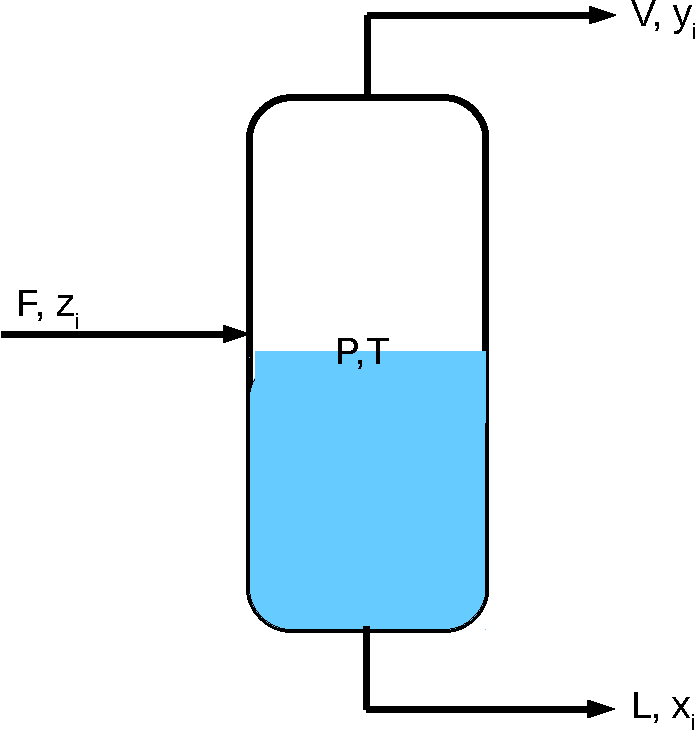
\includegraphics[width=.4\textwidth,clip]{./Figs/FlashDistillation}
     \end{center}
     \caption{Schematic of a flash distillation process.}\label{Chapter:VLE:Fig:Fig06}
  \end{figure}
Flash distillation is a common process in chemical industry to obtain solutions with the required enrichment from a feed-stock. Figure~\ref{Chapter:VLE:Fig:Fig06} shows a schematic of this process, where a liquid stream (\ie with pressure equal to or larger than its bubble point pressure) with molar fraction $F$ and overall composition $z_{i}$ is injected into a separation vessel through a pressure reduction valve. The sudden reduction in pressure leads to partial evaporation (\ie {\it flash}) of the liquid feed resulting in the formation of a vapour and a liquid stream. Vapour and Liquid streams have molar fraction $V$ and $L$, respectively, with compositions of $y_{i}$ and $x_{i}$. 
  The overall mass balance of the system is
  \begin{displaymath}
     F = V + L,
  \end{displaymath}
  for convenience, let's assume $F$ as equal to unity, $F=1$. Similarly, the mass balance for each component $i$ is
  \begin{displaymath}
     z_{i}F = x_{i}L + y_{i}V = x_{i}\left(1-V\right) + y_{i}V.
  \end{displaymath}
  Replacing $x_{i} = \frc{y_{i}}{K_{i}}$ and $F=1$,
  \begin{displaymath}
     z_{i} = \frc{y_{i}}{K_{i}}\left(1-V\right) + y_{i}V \;\;\Longrightarrow \;\;y_{i} = \frc{z_{i}K_{i}}{1+V\left(K_{1}-1\right)}. 
  \end{displaymath}
  As $\summation[y_{i}]{i=1}{\mathcal{C}} = 1$,
         \begin{shaded}
           \begin{equation}
              \summation[\frc{z_{i}K_{i}}{1+V\left(K_{i}-1\right)}]{i=1}{\mathcal{C}} = 1.\label{Chapter:VLE:Eqn:PartialMolarProperties:FlashEquation} 
           \end{equation}
         \end{shaded}
         Solving a $P-T$ flash problem is to \underline{find $V$} that satisfies Eqn.~\ref{Chapter:VLE:Eqn:PartialMolarProperties:FlashEquation}.

  \medskip
   % Example
   \begin{MyExample}{\begin{center}{\bf Example}\end{center}}
     \begin{example}\label{Chapter:VLE:Example5}\citep{Sandler_Book}
       A liquid mixture of 25 mol-$\%$ n-pentane $\left(nC_{5}\right)$, 45 mol-$\%$ n-hexane $\left(nC_{6}\right)$ and 30 mol-$\%$ n-heptane $\left(nC_{7}\right)$ initially at 69$^{\circ}$C and a high pressure, is partially vaporised by isothermically lowering the pressure to  1.013 bar. Calculate the relative amounts of vapour and liquid in equilibrium and compositions.
     \end{example}

% SOLUTION
     \noindent{\bf Solution:}
     This is a typical {\it flash} problem that can be described by Fig.~\ref{Chapter:VLE:Fig:Fig06}. From the given $P_{i}^{\text{sat}}$ relation at 69$^{\circ}$C,
   \begin{displaymath}
        \begin{cases}
            P_{5}^{\text{sat}} = 2.721 \text{ bar},\\ 
            P_{6}^{\text{sat}} = 1.024 \text{ bar},\\
            P_{7}^{\text{sat}} = 0.389 \text{ bar}.
        \end{cases}
   \end{displaymath}
Assuming ideal solution, $K_{i}$ for the three hydrocarbons can be readily obtained,
   \begin{displaymath}
        K_{i} = \frc{P_{i}^{\text{sat}}}{P} = \frc{y_{i}}{x_{i}},
          \begin{cases}
             K_{5} = 2.6861; \\
             K_{6} = 1.0109; \\
             K_{7} = 0.3840
          \end{cases}
   \end{displaymath}
   Therefore,
   \begin{displaymath}
       y_{5} = x_{5}K_{5},\;\;\;y_{6} = x_{6}K_{6},\;\;\;y_{7} = x_{7}K_{7},
   \end{displaymath}
    with the molar fraction constraints,
    \begin{displaymath}
        \begin{cases}
            x_{5}+x_{6}+x_{7} = 1,\\ 
            y_{5}+y_{6}+y_{7} = 1, \\
            F = V + L
        \end{cases}
   \end{displaymath}
   Assuming $F=1$, the mass balance of the individual components in equilibrium are
    \begin{displaymath}
        \begin{cases}
            x_{5}L + y_{5}V = z_{5} = 0.25 \\
            x_{6}L + y_{6}V = z_{6} = 0.45 \\
            x_{7}L + y_{7}V = z_{7} = 0.30            
        \end{cases}
   \end{displaymath}
   these relation can be rewritten as $\left(\text{based on }y_{5}+y_{6}+y_{7} = 1,\; y_{i}=K_{i}x_{i} \;\text{ and } V= 1-L\right)$
    \begin{displaymath}
        \begin{cases}
            x_{5}L + y_{5}V = z_{5} = 0.25 \;\Longrightarrow\; x_{5}\left[L\left(1-K_{5}\right)+K_{5}\right] = 0.25 \\
            x_{6}L + y_{6}V = z_{6} = 0.45 \;\Longrightarrow\; x_{6}\left[L\left(1-K_{6}\right)+K_{6}\right] = 0.45 \\
            x_{7}L + y_{7}V = z_{7} = 0.30 \;\Longrightarrow\; x_{7}\left[L\left(1-K_{7}\right)+K_{7}\right] = 0.30
        \end{cases}
   \end{displaymath}
   Now the molar fraction constraint of the liquid phase $x_{5}+x_{6}+x_{7} = 1$, is
   \begin{displaymath}
        \frc{0.25}{L\left(1-K_{5}\right)+K_{5}} + \frc{0.45}{L\left(1-K_{6}\right)+K_{6}} + \frc{0.30}{L\left(1-K_{7}\right)+K_{7}} = 1
   \end{displaymath}
   This expression has just one unknown, $L$, as a cubic polynomial. Solving with initial guess $L^{\text{guess}}=0.50$ leads to $L=0.5748$.  Now using 
    \begin{displaymath}
        \begin{cases}
            x_{5}L + y_{5}V = z_{5} = 0.25 \;\Longrightarrow\; x_{5}\left[L\left(1-K_{5}\right)+K_{5}\right] = 0.25  \;\Longrightarrow\;  x_{5} = 0.1456 \\
            x_{6}L + y_{6}V = z_{6} = 0.45 \;\Longrightarrow\; x_{6}\left[L\left(1-K_{6}\right)+K_{6}\right] = 0.45  \;\Longrightarrow\;  x_{6} = 0.4479 \\
            x_{7}L + y_{7}V = z_{7} = 0.30 \;\Longrightarrow\; x_{7}\left[L\left(1-K_{7}\right)+K_{7}\right] = 0.30  \;\Longrightarrow\;  x_{7} = 0.4065 
        \end{cases}
   \end{displaymath}
   leading to $\summation[x_{i}]{i}{} = 1.0000$. Molar fraction of the vapour phase is $V= 1-L=0.4252$, resulting in
    \begin{displaymath}
        \begin{cases}
            y_{5} = K_{5}x_{5} \;\Longrightarrow\; y_{5} = 0.3911 \\
            y_{6} = K_{6}x_{6} \;\Longrightarrow\; y_{6} = 0.4528 \\
            y_{7} = K_{7}x_{7} \;\Longrightarrow\; y_{7} = 0.1561 
        \end{cases}
   \end{displaymath}
    with $\summation[y_{i}]{i}{} = 1.0000$
   \end{MyExample}
   

\clearpage   
\begin{FinalSummaryBlock}{Summary}
     Concepts introduced in this chapter are relatively simple but far reaching. They are cornerstone for the remaining of this notes and for fundamental chemical thermodynamics. An extension of total derivative to multi-component systems led to the equilibrium criteria for general multiphase ($\mathcal{P}\ge2$) and multi-component ($\mathcal{C}\ge2$) mixtures.
    \begin{itemize}
       \item Initial definition and discussion of excess properties (Eqn.~\ref{Chapter:VLE:Eqn:ExcessProperties1a});
       \item Definition of chemical potential as the partial molar Gibbs free energy (Eqn.~\ref{Chapter:VLE:Eqn:ChemPotentialDef1b}) and development of a fundamental relation for multi-component systems (Eqn.~\ref{Chapter:VLE:Eqn:ChemPotentialDef1d});
       \item Chemical equilibrium can be assessed \wrt thermodynamic conditions as stated in Table~\ref{Chapter:VLE:Table:TableEquilibriumCriteria};
       \item In closed systems at constant pressure and temperature conditions, the criterion for equilibrium is that the Gibbs free energy is the minimum which leads to equality of chemical potential of each component at all phases (Eqn.~\ref{Chapter:VLE:EqnChemPotentialDef1c3});
       \item Multi-component VLE problems (\ie $\mathcal{C}\ge 2$ and $\mathcal{P}=2$) can be represented by $P-T-x_{i}y_{i}$ phase diagrams, where critical pressure and temperature (for individual components and the mixtures), liquid and vapour saturation lines, bubble and dew points can be identified;
       \item Although compositions, temperatures and pressures can be obtained from graphical representation (2-/3-D) of phase equilibrium, this is not very convenient and numerical models were develop to represent the partition of components in both phases in equilibrium;
       \item Raoult's law (Eqn.~\ref{Chapter:VLE:Eqn:RaoultLaw}) is an idealisation of the components' partition between vapour and liquid phases assuming limited molecular forces (\eg attractive and repulsive) act in the liquid phase;
       \item Henry's law (Eqn.~\ref{Chapter:VLE:Eqn:HenryLaw}) is applied to gases solubilised at low concentrations in liquid solutions;
       \item K-value models (Eqn.~\ref{Chapter:VLE:Eqn:KValue}) were mostly developed for petro-chemical industry to help quickly assess concentrations of (light) hydrocarbons in vapour and liquid phases;
       \item Dew and bubble coordinates (pressure, temperature and compositions) in typical industrial applications are discussed in Section~\ref{Chapter:VLE:Section:IndApplications};
       \item Depending on known conditions, four main problems may arise:
\begin{center}
   \begin{tabular}{|l c c|}
      \hline 
      $\mathbf{VLE}$ {\bf Problem} & {\bf Specified Variables} &  {\bf Computed Variables} \\  
      \hline
          {\bf Bubble Pressure}        &  $T$ and $x_{i}$           &   $P$ and $y_{i}$          \\
          {\bf Dew Pressure}           &  $T$ and $y_{i}$           &   $P$ and $x_{i}$          \\
          {\bf Bubble Temperature}     &  $P$ and $x_{i}$           &   $T$ and $y_{i}$          \\
          {\bf Dew Temperature}        &  $P$ and $y_{i}$           &   $T$ and $x_{i}$          \\     
      \hline
   \end{tabular}
\end{center}
    \end{itemize}
\end{FinalSummaryBlock}
